%% CSSP manuscript draft -- Springer Nature sn-jnl template (pdflatex, numbered references)
\documentclass[pdflatex,sn-mathphys-num]{sn-jnl}

\usepackage{graphicx}%
\usepackage{multirow}%
\usepackage{amsmath,amssymb,amsfonts}%
\usepackage{amsthm}%
\usepackage{mathrsfs}%
\usepackage[title]{appendix}%
\usepackage{xcolor}%
\usepackage{textcomp}%
\usepackage{manyfoot}%
\usepackage{booktabs}%
\usepackage{algorithm}%
\usepackage{algorithmicx}%
\usepackage{algpseudocode}%
\usepackage{listings}%
\usepackage{array}%
\usepackage{tikz}%
\usetikzlibrary{arrows.meta,positioning,calc}%

\theoremstyle{thmstyleone}%
\newtheorem{theorem}{Theorem}%
\newtheorem{proposition}[theorem]{Proposition}%
\newtheorem{lemma}[theorem]{Lemma}%
\newtheorem{corollary}[theorem]{Corollary}%
\theoremstyle{thmstyletwo}%
\newtheorem{example}{Example}%
\newtheorem{remark}{Remark}%
\theoremstyle{thmstylethree}%
\newtheorem{definition}{Definition}%

\raggedbottom

%% ---------------------------------------------------------------- macros
\newcommand{\Ts}{T_{\mathrm{s}}}
\newcommand{\cd}{c_{\mathrm{d}}}
\newcommand{\sd}{s_{\mathrm{d}}}
\newcommand{\ulo}{u_{\mathrm{lo}}}
\newcommand{\uhi}{u_{\mathrm{hi}}}
\newcommand{\xlo}{\xi_{\mathrm{lo}}}
\newcommand{\xhi}{\xi_{\mathrm{hi}}}
\newcommand{\gh}{\hat g}
\newcommand{\Hh}{\hat H}
\newcommand{\Op}[2]{{}^{\mathrm{#1}}\!\Delta^{#2}}
\newcommand{\WA}{W_{\mathrm A}}
\newcommand{\WB}{W_{\mathrm B}}
\newcommand{\WD}{W_{\mathrm D}}
\newcommand{\WE}{W_{\mathrm E}}
\newcommand{\Beta}{\mathrm{B}}
\newcommand{\eps}{\varepsilon}
\newcommand{\pending}[1]{\textcolor{red}{[#1]}}

\begin{document}

\title[Variable-order operators from one fixed-pole bank]{Definition-Consistent Variable-Order Fractional Operators from a Single Fixed-Pole Bank: Structure, Design Rule, and Fixed-Point Realization}

%% TODO: author names, affiliations and e-mail addresses
\author*[1]{\fnm{First} \sur{Author}}\email{first.author@example.org}
\author[1]{\fnm{Second} \sur{Author}}\email{second.author@example.org}
\affil*[1]{\orgdiv{Department}, \orgname{Institution}, \orgaddress{\city{City}, \country{Country}}}

\abstract{Variable-order (VO) fractional operators have several inequivalent definitions, which differ in how past values of the order enter the memory. Practical realizations are finite-dimensional, and when their coefficients are switched as the order varies it is generally unclear which definition they implement. We show that an exact switching state map between two realizations exists only if the realizations are similar, so realizations whose poles move with the order cannot implement the A- or B-type Gr\"unwald--Letnikov definitions under switching. Least-squares state maps narrow the gap in floating point, but they are dense, depend on the input class and lose three to nine orders of magnitude of accuracy in 24-bit fixed point. Instead, a Beta-integral representation realizes the Gr\"unwald--Letnikov weights with order-independent discrete poles. With the order in the output weights this bank is the A-type, and with the order in the input weights the B-type, for every order sequence and up to the frozen-order quadrature error. Inverting the same bank gives the recursive D- and E-types with exact duality at $O(K)$ cost per sample. A fit-free analytic error model sets the bank size and met all 400 specifications of a sealed holdout. A derivative bank has a stable inverse if and only if its realized DC gain is positive, which a small DC floor guarantees. A bit-exact fixed-point Verilog core changes order and type at every sample through a ROM address only. As an application, the bank streams multifractional Brownian motion of Riemann--Liouville type and its B-type variant for $0<H<1$.}

\keywords{variable-order fractional calculus, Gr\"unwald--Letnikov, diffusive representation, fixed-pole approximation, duality, fixed-point hardware, multifractional Brownian motion}

\maketitle

%% =====================================================================
\section{Introduction}\label{sec:intro}

Fractional-order operators describe systems whose memory decays as a power law. When the decay exponent itself changes in time, the natural model is a variable-order (VO) operator, whose order $\alpha(t)$ is a function of time~\cite{samko1993,lorenzo2002,sun2019,patnaik2020}. Unlike the constant-order case, the generalization is not unique. Different ways of letting the order enter the memory kernel give operators that coincide for constant order but differ as soon as the order changes~\cite{lorenzo2002,valerio2011,garrappa2021}.

For Gr\"unwald--Letnikov (GL) operators, Sierociuk et al.\ use four types~\cite{sierociuk2015amm,sierociuk2015cssp,malesza2016,sierociuk2020}:
\begin{itemize}
\item the A-type weights the whole history with the current order;
\item the B-type weights each past sample with the order that was active when the sample entered;
\item the recursive D- and E-types are the inverses of the A- and B-types of opposite order~\cite{sierociuk2015cssp,sierociuk2016cssp,sierociuk2020}.
\end{itemize}
After a single order switch these definitions can differ by as much as the output itself (relative differences of 0.5 to 1.35 in Sect.~\ref{sec:results}). The choice of definition is therefore part of the model, not a detail of the numerics.

Practical realizations of fractional operators are finite-dimensional. Constant-order operators are approximated by rational transfer functions, most often by Oustaloup's recursive distribution of poles and zeros~\cite{oustaloup2000}, Charef's fractional power pole~\cite{charef1992} and related schemes~\cite{vinagre2000}. The poles and zeros of these approximations move with the order. Fixed-pole approximations with order-independent poles have been proposed for constant orders~\cite{wei2016,wei2019,wei2021}. Diffusive, infinite-state and sum-of-exponentials representations also lead to realizations with fixed nodes~\cite{montseny1998,trigeassou2012,baffet2017,jiang2017,diethelm2023}.

When the order varies, a constant-order realization can be switched between orders, either by switching circuits or by changing its coefficients while keeping its state (a ``hot swap''). In our previous work on a constant-order FPGA core~\cite{tcas_submission}, such swaps produced short, bounded transients; which VO operator they implement was not addressed. Section~\ref{sec:related} reviews how existing realizations handle a varying order.

This leaves two open questions:
\begin{enumerate}
\item Given an arbitrary order sequence, which VO definition does a finite-dimensional realization implement?
\item Can the structure of the realization select the definition at no extra cost per sample?
\end{enumerate}
This paper answers both for GL operators of order $-1<\alpha<1$. The contributions are:
\begin{enumerate}
\item \emph{Necessity.} An exact switching state map exists only between similar realizations (Theorem~\ref{thm:necessity}). Realizations with order-dependent poles therefore cannot implement the A- or B-type exactly at a switch, with or without a state map. Least-squares maps reduce the error in floating point. However, they need a dense $S\times S$ matrix per pair of orders, depend on the input class, and lose three to nine orders of magnitude of accuracy in 24-bit fixed point (Sect.~\ref{sec:res-maps}).
\item \emph{Definition by structure.} Order-independent exponents have already been used for the A-type VO Caputo derivative in fast numerical solvers~\cite{zhang2022esa,zhang2022fast}. We show that, in a fixed-pole structure, the place of the order selects the definition. A Beta-integral representation of the GL weights gives a discrete bank with order-independent poles. With the order in the output weights the bank realizes the A-type, and with the order in the input weights the B-type. This holds for every order sequence, up to the frozen-order quadrature error (Proposition~\ref{prop:structure}); the B-type thus costs $O(K)$ per sample as well. Algebraic inversion of the same bank gives the D- and E-types with exact duality at the same cost, and solves VO relaxation equations of all four types (Proposition~\ref{prop:inverse}). In analog form, a direct realization of the D-type has been considered impractical~\cite{sierociuk2020}.
\item \emph{Fit-free design.} An analytic error model with three closed-form terms sets the bank size and pole range from the tolerance, the memory length and the order range. On a sealed holdout of 400 random specifications the rule met every tolerance (Sects.~\ref{sec:design} and~\ref{sec:res-rule}).
\item \emph{Inverse stability.} The inverse of a derivative bank is stable if and only if its realized DC gain is positive (Proposition~\ref{prop:stability}). This condition is tested through an exact sign rather than through eigenvalues. A DC floor applied through the delay mode guarantees it, also after coefficient quantization.
\item \emph{Hardware.} A time-multiplexed fixed-point core realizes all four types. Order and type are per-sample inputs, and changing them only changes a ROM address. The core is bit-exact with its golden model (94\,208 vectors, no mismatch). Word lengths for two operating envelopes and synthesis estimates are reported.
\item \emph{Application.} The bank streams multifractional Brownian motion (mBm) of Riemann--Liouville type, which is an A-type integral of white noise, and its B-type counterpart, which is the memory-multifractional Brownian motion of~\cite{wang2023mmfbm} up to normalization, for $0<H<1$. One bank suffices because an integer split is exact when placed according to the type (Proposition~\ref{prop:split}).
\end{enumerate}

Section~\ref{sec:related} reviews related work. Section~\ref{sec:prelim} recalls the definitions and their duality. Section~\ref{sec:bank} builds the continuous- and discrete-time fixed-pole banks, Section~\ref{sec:structure} proves the structural results, and Section~\ref{sec:design} gives the error model, the design rule and the stability result. Section~\ref{sec:results} reports the numerical experiments, Section~\ref{sec:hw} the fixed-point core, and Section~\ref{sec:mbm} the mBm application. Section~\ref{sec:discussion} discusses limitations. All code, seeds and results are available (see the Declarations).

\subsection{Related work}\label{sec:related}

The search behind this section is documented in the repository: protocol, queries, screening decisions and data extraction. It used Crossref and arXiv and was complemented by snowballing. Table~\ref{tab:related} summarizes how existing realizations treat a varying order.

\paragraph{Analog realizations.} Most analog VO realizations switch between two or three constant-order circuits~\cite{sierociuk2013tcst,macias2020,zhou2019}, as noted in~\cite{aricioglu2025}. Sierociuk et al.\ made the link between structure and definition explicit for switching:
\begin{itemize}
\item a serial cascade in which a block of complementary order is pre-connected at every switch is equivalent to the B-type~\cite{sierociuk2015amm};
\item switching strategies for the recursive types follow from duality~\cite{sierociuk2015cssp,malesza2016,sierociuk2016ecc,sierociuk2014bpas};
\item a parallel scheme replaced the serial one, which could not be built in practice~\cite{sierociuk2018amc}.
\end{itemize}
The D-type was found impractical to realize directly, because two ideal operators of opposite orders cannot be connected in series with electronic elements~\cite{sierociuk2020}. These schemes add or switch constant-order blocks, so their size grows with the number of distinct switches. Ar{\i}c{\i}o{\u{g}}lu realized a smoothly varying order with a single transfer function~\cite{aricioglu2025}. This restricts the method to the only linear time-invariant definition of Lorenzo and Hartley~\cite{lorenzo2002}. Electronically tunable fractional-order elements and filters~\cite{tsirimokou2017,charef2012,yu2022} and variable fractional-order digital differentiators and integrators~\cite{tseng2006,tseng2008,charef2012sivp} make the order an adjustable parameter of a constant-order design. Their behaviour while the order changes is not analysed.

\paragraph{Digital and hardware realizations.} Tolba et al.\ realized GL operators on an FPGA with an order that can be reconfigured at run time, and used them in a VO chaotic oscillator~\cite{tolba2020}. A direct GL convolution with current-order weights has fixed poles (all at the origin) and its order in the output weights. By the argument of Proposition~\ref{prop:structure} below it is therefore an A-type operator, with a memory and a cost per sample proportional to its length. Discrete-time VO controllers evaluate GL VO differences directly~\cite{mozyrska2019}, at a cost that grows with the memory.

\paragraph{Fixed nodes for variable orders.} The work closest to ours comes from fast solvers for VO time-fractional equations. Zhang, Fang and Sun approximate the VO Caputo derivative, with the order taken at the current time, by an exponential sum whose exponents do not change between time levels~\cite{zhang2022esa,zhang2022fast}. Huang et al.\ give a unified sum-of-exponentials framework for constant and variable orders~\cite{huang2022unified}. These works share the order-independent nodes with the present paper. However, they treat only the A-type, in continuous time and inside an L1-type discretization. They do not address the B-, D- or E-types, a design rule over the whole order range, or hardware. For the hidden-memory VO derivative, whose order is evaluated at the integration variable as in the B-type, the fast method we found uses Taylor expansions and hierarchical matrices at $O(N\log N)$ total cost~\cite{jia2022}.

\paragraph{State and transients.} Transients caused by coefficient changes in recursive filters are a classical topic~\cite{zetterberg1988,valimaki1998}. The meaning of the state of a fractional system has been discussed in the context of initialization~\cite{lorenzo2008,trigeassou2012,sabatier2014}. Neither line asks which VO definition a switched realization implements.

\begin{table}[t]
\caption{How existing realizations treat a varying order. ``Inferred'' marks entries obtained by applying Proposition~\ref{prop:structure} or Theorem~\ref{thm:necessity} to the described structure}\label{tab:related}
\footnotesize\setlength{\tabcolsep}{3pt}
\begin{tabular}{@{}>{\raggedright\arraybackslash}p{0.19\textwidth}>{\raggedright\arraybackslash}p{0.27\textwidth}>{\raggedright\arraybackslash}p{0.17\textwidth}>{\raggedright\arraybackslash}p{0.16\textwidth}>{\raggedright\arraybackslash}p{0.14\textwidth}@{}}
\toprule
Work & Structure & Definition & Order changes & Cost per sample\\
\midrule
serial switching~\cite{sierociuk2015amm} & analog; complementary-order block added at each switch & B & any number of switches & grows with switches\\
recursive, parallel schemes~\cite{sierociuk2015cssp,sierociuk2018amc,sierociuk2020} & analog; switched constant-order ladders & D; B; B$\leftrightarrow$D & a few switches & ---\\
\cite{aricioglu2025} & analog; one transfer function & LTI (third) type of~\cite{lorenzo2002} & smooth $\alpha(t)$ & fixed\\
tunable elements, filters~\cite{tsirimokou2017,charef2012,yu2022,tseng2006,charef2012sivp} & order-dependent coefficients & not analysed (FIR: A, inferred) & re-tuning & ---\\
FPGA GL~\cite{tolba2020} & direct GL convolution & A (inferred) & at run time & $O(L)$, $L$ = memory\\
hot-swapped Oustaloup (Sect.~\ref{sec:results}) & moving poles, state kept & none exactly (Thm.~\ref{thm:necessity}) & any & $O(S)$\\
exponential sums~\cite{zhang2022esa,huang2022unified} & fixed exponents, continuous-time Caputo & A & any $\alpha(t)\in(0,1)$ & $O(\log^2 n)$\\
hidden memory~\cite{jia2022} & Taylor / hierarchical matrices & B-like (Caputo) & any & $O(N\log N)$ in total\\
this work & discrete fixed-pole bank & A, B; D, E by inversion & every sample & $O(K)$, $K\approx20$--$50$\\
\botrule
\end{tabular}
\end{table}

%% =====================================================================
\section{Variable-order Gr\"unwald--Letnikov operators}\label{sec:prelim}

\subsection{Definitions}

Let $\Ts$ be the sampling period and $\alpha_n\in(-1,1)$ the order at sample $n\ge 0$. An order $\alpha>0$ is a derivative, $\alpha<0$ an integral and $\alpha=0$ the identity. Signals vanish for $n<0$. We write
\begin{equation}
w_r(a)=(-1)^r\binom{a}{r}=w_{r-1}(a)\,\frac{r-1-a}{r},\quad w_0=1,\qquad g_r(a)=\Ts^{-a}\,w_r(a).\label{eq:glw}
\end{equation}

\begin{definition}[VO GL operators~\cite{sierociuk2015amm,sierociuk2015cssp,sierociuk2020}]\label{def:types}
For an input $x$ and an order sequence $\alpha$,
\begin{align}
\big(\Op{A}{\alpha}x\big)_n &= \sum_{r=0}^{n} g_r(\alpha_n)\,x_{n-r}, \label{eq:A}\\
\big(\Op{B}{\alpha}x\big)_n &= \sum_{r=0}^{n} g_r(\alpha_{n-r})\,x_{n-r}, \label{eq:B}\\
z_n=\big(\Op{D}{\alpha}x\big)_n &= \Ts^{-\alpha_n}x_n-\sum_{r=1}^{n} w_r(-\alpha_n)\,z_{n-r}, \label{eq:D}\\
z_n=\big(\Op{E}{\alpha}x\big)_n &= \Ts^{-\alpha_n}x_n-\sum_{r=1}^{n} w_r(-\alpha_{n-r})\,\Ts^{\alpha_{n-r}-\alpha_n}\,z_{n-r}. \label{eq:E}
\end{align}
\end{definition}

The A-type has no memory of past orders: a change of $\alpha_n$ immediately reweights the entire history. The B-type keeps each sample with the weight sequence of its own entry order. For a constant order all four types coincide. In~\cite{sierociuk2015amm} the A- and B-types are the first and second types. Their third type indexes the order by the lag, which gives a time-invariant operator. Lorenzo and Hartley~\cite{lorenzo2002} and Val\'erio and S\'a da Costa~\cite{valerio2011} list further variants, and~\cite{malesza2019} exploits the duality below to solve VO equations analytically.

\subsection{Matrix form and duality}

On a horizon of $N$ samples the A- and B-types are lower-triangular matrices,
\begin{equation}
[\WA(\alpha)]_{n,j}=g_{n-j}(\alpha_n),\qquad [\WB(\alpha)]_{n,j}=g_{n-j}(\alpha_j),\qquad 0\le j\le n<N.\label{eq:matrix}
\end{equation}
Row $n$ of $\WA(-\alpha)z=x$ reads $\Ts^{\alpha_n}z_n+\Ts^{\alpha_n}\sum_{r\ge1}w_r(-\alpha_n)z_{n-r}=x_n$, which is~\eqref{eq:D}. Row $n$ of $\WB(-\alpha)z=x$ is~\eqref{eq:E}. Hence
\begin{equation}
\WD(\alpha)=\WA(-\alpha)^{-1},\qquad \WE(\alpha)=\WB(-\alpha)^{-1},\label{eq:duality}
\end{equation}
which is the duality of~\cite{sierociuk2015cssp,sierociuk2016cssp,sierociuk2020}. For a varying order, the A-types (or the B-types) of opposite orders are not inverses of each other: $\WA(\alpha)\WA(-\alpha)\neq I$ in general. The recursive types are therefore genuinely different operators. Section~\ref{sec:res-types} quantifies these relations numerically.

\subsection{Continuous-time references}

For the continuous-time experiments we use the step responses of the A- and B-types. With $F(t,a)=t^{-a}/\Gamma(1-a)$, the step response of the constant-order operator $s^{a}$, they are
\begin{align}
y_{\mathrm A}(t) &= F\big(t,\alpha(t)\big), \label{eq:stepA}\\
y_{\mathrm B}(t) &= F\big(t,\alpha(0)\big)+\int_0^t \partial_a F\big(t-\tau,\alpha(\tau)\big)\,\dot\alpha(\tau)\,\mathrm d\tau. \label{eq:stepB}
\end{align}
Equation~\eqref{eq:stepB} is derived in Appendix~\ref{app:stepB}. For a piecewise-constant order with switches at $T_i$, \eqref{eq:stepB} reduces to $F(t,\alpha_0)+\sum_i\big[F(t-T_i,\alpha_i)-F(t-T_i,\alpha_{i-1})\big]$.

\subsection{Diffusive representation}

For $0<a<1$ and $S_a=\sin(\pi a)/\pi$~\cite{montseny1998,diethelm2023},
\begin{equation}
s^{-a}=S_a\int_0^\infty \frac{\xi^{-a}}{s+\xi}\,\mathrm d\xi,\qquad s^{a}=S_a\int_0^\infty \xi^{a-1}\,\frac{s}{s+\xi}\,\mathrm d\xi.\label{eq:diffusive}
\end{equation}
The order enters only through the density in $\xi$; the pole $-\xi$ of each element does not depend on it. This is the property the paper builds on.

%% =====================================================================
\section{Fixed-pole banks}\label{sec:bank}

\subsection{Continuous time}

Let $\xi_k=\xlo e^{kh}$, $k=0,\dots,K-1$, be a geometric grid with spacing $h$ in $\ln\xi$, and apply the trapezoidal rule to~\eqref{eq:diffusive}. Every order is then written on the same bank of unit-DC-gain states $\dot x_k=-\xi_k x_k+\xi_k u$:
\begin{equation}
H_\alpha(s)=d(\alpha)+\sum_{k=0}^{K-1} m_k(\alpha)\,\frac{\xi_k}{s+\xi_k}.\label{eq:ctbank}
\end{equation}
For an integral, $\alpha=-a<0$, the weights are $m_k=hS_a\xi_k^{-a}$. For a derivative, $\alpha=a>0$, we use $s/(s+\xi)=1-\xi/(s+\xi)$: then $m_k=-v_k$ with $v_k=hS_a\xi_k^{a}$, and the feedthrough collects $\sum_k v_k$. The two truncated tails are closed by the geometric series of the virtual trapezoid nodes beyond the grid:
\begin{itemize}
\item one tail is lumped onto the outermost pole: $m_0\mathrel{+}=S_a\xlo^{-a}G_h(1-a)$ for integrals, $v_{K-1}\mathrel{+}=S_a\xhi^{a}G_h(1-a)$ for derivatives;
\item the other becomes feedthrough: $d=S_a\xhi^{-a}G_h(a)$ for integrals, $d=\sum_k v_k+S_a\xlo^{a}G_h(a)$ for derivatives.
\end{itemize}
Here
\begin{equation}
G_h(p)=\sum_{j\ge1}h\,e^{-pjh}=\frac{h}{e^{ph}-1},\qquad H_h(p,q)=G_h(p)-G_h(q).\label{eq:G}
\end{equation}
All nodes carry the full weight $h$. The bank therefore equals the infinite trapezoidal rule except for asymptotic tail residuals, and no $O(h^2)$ endpoint term appears. At $\alpha=0$ the bank is the identity ($m=0$, $d=1$). Since $S_aG_h(a)\to1$ as $a\to0$, the coefficients are continuous when the order crosses zero.

\subsection{Discrete time: a Beta-integral representation of the GL weights}

Sampling the continuous-time bank introduces a second error, because modes faster than $1/\Ts$ respond to the staircase of a sampled order (Sect.~\ref{sec:res-def}). We therefore realize the GL weights~\eqref{eq:glw} themselves.

\begin{lemma}\label{lem:beta}
For $r\ge1$ and $-1<a<1$,
\begin{equation}
w_r(a)=-S_a\,\Beta(r-a,1+a)=-S_a\int_0^1\theta^{\,r-a-1}(1-\theta)^{a}\,\mathrm d\theta.\label{eq:beta}
\end{equation}
\end{lemma}
\begin{proof}
$w_r(a)=\Gamma(r-a)/\big(\Gamma(-a)\Gamma(r+1)\big)$ and $\Beta(r-a,1+a)=\Gamma(r-a)\Gamma(1+a)/\Gamma(r+1)$. The reflection formula gives $\Gamma(-a)\Gamma(1+a)=-\pi/\sin(\pi a)$. For $a=0$ both sides vanish.
\end{proof}

The weights are thus a superposition of geometric sequences $\theta^{r}$ with an order-dependent density. With $\theta=e^{-u}$ and $u=e^{x}$,
\begin{equation}
w_r(a)=-S_a\int_{-\infty}^{\infty}\varphi_a\big(e^{x}\big)\,e^{-(r-1)e^{x}}\,\mathrm dx,\qquad \varphi_a(u)=u\,e^{-(1-a)u}\big(1-e^{-u}\big)^{a}.\label{eq:betax}
\end{equation}
The trapezoidal rule on $u_k=\ulo e^{kh}$, $k=0,\dots,K-1$, gives order-independent discrete poles $\theta_k=e^{-u_k}$. With $u_k=\xi_k\Ts$, each $\theta_k$ is the zero-order-hold image of the continuous-time pole $-\xi_k$. The realized weights are
\begin{equation}
\begin{aligned}
\gh_0(a)&=\Ts^{-a},\qquad \gh_r(a)=\delta_{r1}\,\cd(a)+\sum_{k=0}^{K-1}c_k(a)\,\theta_k^{\,r-1}\quad(r\ge1),\\
c_k(a)&=-S_a\Ts^{-a}h\,\varphi_a(u_k),
\end{aligned}\label{eq:dtweights}
\end{equation}
and the frozen-order transfer function is
\begin{equation}
\Hh_a(z)=\sum_{r\ge0}\gh_r(a)z^{-r}=\Ts^{-a}+\frac{\cd(a)}{z}+\sum_{k=0}^{K-1}\frac{c_k(a)}{z-\theta_k}.\label{eq:dtH}
\end{equation}

The tails are again closed by virtual trapezoid nodes:
\begin{itemize}
\item the nodes below the grid ($\theta\approx1$) are lumped onto $\theta_0$, matched at $r=1$: $c_0\mathrel{+}=-S_a\Ts^{-a}\sum_{j\ge1}h\varphi_a(\ulo e^{-jh})$;
\item the nodes above the grid ($\theta\approx0$) contribute only at $r=1$ and form the \emph{delay mode} (a pole at $\theta=0$): $\cd=-S_a\Ts^{-a}\sum_{j\ge1}h\varphi_a(\uhi e^{jh})$.
\end{itemize}
Since $\varphi_a>0$, all residues have the sign of $-a$: integral banks have positive residues and derivative banks negative ones (before the DC floor of Sect.~\ref{sec:stability}). The weight $\gh_0$ is exact, and at $a=0$ the bank is exactly the identity. As $a\to0$ all residues vanish continuously, so the bank crosses the order zero without any special case.

\subsection{Order schedules}

The bank has $K$ first-order states $s_k$ and the delay state $\sd$. The order can be scheduled in two places (Fig.~\ref{fig:bank}), the output schedule (OS) and the input schedule (IS):
\begin{equation}
\text{OS:}\quad
\begin{aligned}
s_k[n+1]&=\theta_k s_k[n]+v_n,\qquad \sd[n+1]=v_n,\\
y_n&=\Ts^{-\alpha_n}v_n+\underbrace{\cd(\alpha_n)\,\sd[n]+\textstyle\sum_k c_k(\alpha_n)\,s_k[n]}_{\eta_n},
\end{aligned}\label{eq:os}
\end{equation}
\begin{equation}
\text{IS:}\quad
\begin{aligned}
s_k[n+1]&=\theta_k s_k[n]+c_k(\alpha_n)\,v_n,\qquad \sd[n+1]=\cd(\alpha_n)\,v_n,\\
y_n&=\Ts^{-\alpha_n}v_n+\underbrace{\sd[n]+\textstyle\sum_k s_k[n]}_{\eta_n}.
\end{aligned}\label{eq:is}
\end{equation}
In both cases $y_n=\gh_0(\alpha_n)v_n+\eta_n$, where the history $\eta_n$ depends only on $v_0,\dots,v_{n-1}$ because the poles do not depend on the order. Changing the order never touches the state.

\begin{figure}[t]
\centering
\resizebox{\textwidth}{!}{%
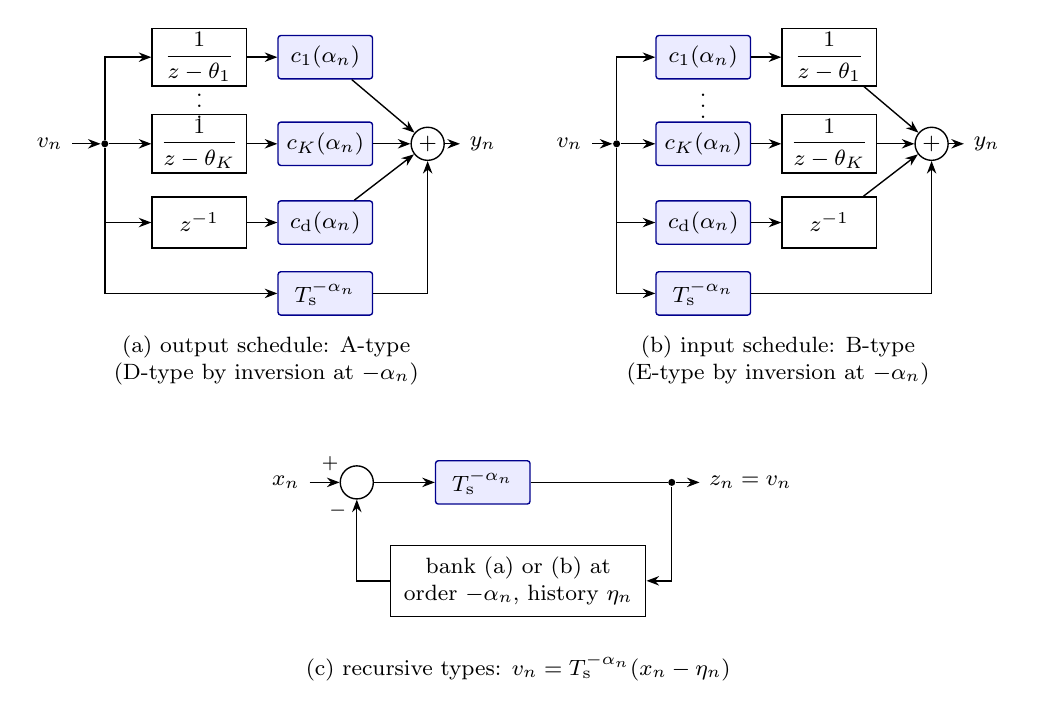
\begin{tikzpicture}[>={Stealth[length=1.6mm]}, font=\footnotesize, line width=0.5pt,
  blk/.style={draw, minimum height=6.5mm, minimum width=12mm, inner sep=1.5pt},
  gain/.style={draw=blue!55!black, fill=blue!8, rounded corners=1pt, minimum height=5.5mm, minimum width=12mm, inner sep=1pt},
  sum/.style={draw, circle, minimum size=4.2mm, inner sep=0pt},
  dot/.style={circle, fill, inner sep=0.9pt}]
%% (a) output schedule
\begin{scope}
\node (in) at (0,0) {$v_n$};
\node[dot] (sp) at (0.7,0) {};
\node[blk] (b1) at (1.9,1.1) {$\dfrac{1}{z-\theta_1}$};
\node at (1.9,0.58) {$\vdots$};
\node[blk] (bK) at (1.9,0.0) {$\dfrac{1}{z-\theta_K}$};
\node[blk] (bd) at (1.9,-1.0) {$z^{-1}$};
\node[gain] (c1) at (3.5,1.1) {$c_1(\alpha_n)$};
\node[gain] (cK) at (3.5,0.0) {$c_K(\alpha_n)$};
\node[gain] (cd) at (3.5,-1.0) {$c_{\mathrm d}(\alpha_n)$};
\node[gain] (g0) at (3.5,-1.9) {$\Ts^{-\alpha_n}$};
\node[sum] (S) at (4.8,0) {$+$};
\node (out) at (5.5,0) {$y_n$};
\draw[->] (in) -- (sp);
\draw[->] (sp) |- (b1);
\draw[->] (sp) -- (bK);
\draw[->] (sp) |- (bd);
\draw[->] (sp) |- (g0);
\draw[->] (b1) -- (c1);
\draw[->] (bK) -- (cK);
\draw[->] (bd) -- (cd);
\draw[->] (c1) -- (S);
\draw[->] (cK) -- (S);
\draw[->] (cd) -- (S);
\draw[->] (g0) -| (S);
\draw[->] (S) -- (out);
\node[align=center] at (2.75,-2.75) {(a) output schedule: A-type\\(D-type by inversion at $-\alpha_n$)};
\end{scope}
%% (b) input schedule
\begin{scope}[xshift=6.6cm]
\node (in) at (0,0) {$v_n$};
\node[dot] (sp) at (0.6,0) {};
\node[gain] (c1) at (1.7,1.1) {$c_1(\alpha_n)$};
\node at (1.7,0.58) {$\vdots$};
\node[gain] (cK) at (1.7,0.0) {$c_K(\alpha_n)$};
\node[gain] (cd) at (1.7,-1.0) {$c_{\mathrm d}(\alpha_n)$};
\node[gain] (g0) at (1.7,-1.9) {$\Ts^{-\alpha_n}$};
\node[blk] (b1) at (3.3,1.1) {$\dfrac{1}{z-\theta_1}$};
\node[blk] (bK) at (3.3,0.0) {$\dfrac{1}{z-\theta_K}$};
\node[blk] (bd) at (3.3,-1.0) {$z^{-1}$};
\node[sum] (S) at (4.6,0) {$+$};
\node (out) at (5.3,0) {$y_n$};
\draw[->] (in) -- (sp);
\draw[->] (sp) |- (c1);
\draw[->] (sp) -- (cK);
\draw[->] (sp) |- (cd);
\draw[->] (sp) |- (g0);
\draw[->] (c1) -- (b1);
\draw[->] (cK) -- (bK);
\draw[->] (cd) -- (bd);
\draw[->] (b1) -- (S);
\draw[->] (bK) -- (S);
\draw[->] (bd) -- (S);
\draw[->] (g0) -| (S);
\draw[->] (S) -- (out);
\node[align=center] at (2.65,-2.75) {(b) input schedule: B-type\\(E-type by inversion at $-\alpha_n$)};
\end{scope}
%% (c) inversion
\begin{scope}[xshift=3.6cm, yshift=-4.3cm]
\node (in) at (-0.6,0) {$x_n$};
\node[sum] (S) at (0.3,0) {};
\node at ($(S)+(-0.34,0.24)$) {\scriptsize $+$};
\node at ($(S)+(-0.24,-0.36)$) {\scriptsize $-$};
\node[gain] (g) at (1.9,0) {$\Ts^{-\alpha_n}$};
\node[dot] (tap) at (4.3,0) {};
\node (out) at (5.3,0) {$z_n=v_n$};
\node[draw, align=center, text width=31mm, minimum height=9mm, inner sep=2pt] (bank) at (2.35,-1.25) {bank (a) or (b) at order $-\alpha_n$, history $\eta_n$};
\draw[->] (in) -- (S);
\draw[->] (S) -- (g);
\draw[->] (g) -- (tap) -- (out);
\draw[->] (tap) |- (bank.east);
\draw[->] (bank.west) -| (S.south);
\node[align=center] at (2.35,-2.35) {(c) recursive types: $v_n=\Ts^{-\alpha_n}(x_n-\eta_n)$};
\end{scope}
\end{tikzpicture}}
\caption{Fixed-pole bank. The poles $\theta_k$ and the delay $z^{-1}$ are common to every order; only the shaded weights depend on $\alpha_n$. (a) Order in the output weights. (b) Order in the input weights. (c) The recursive types: the history $\eta_n$ of bank (a) or (b), run at order $-\alpha_n$, is removed and the result is scaled by $1/\gh_0(-\alpha_n)=\Ts^{-\alpha_n}$. The feedthrough of the bank at order $-\alpha_n$ is $\Ts^{\alpha_n}$, which is why the gain in (c) is $\Ts^{-\alpha_n}$}\label{fig:bank}
\end{figure}

%% =====================================================================
\section{Definition by structure}\label{sec:structure}

\begin{proposition}[Definition by structure]\label{prop:structure}
For every order sequence $(\alpha_n)\subset(-1,1)$, every input $v$ and zero initial state,
\begin{equation}
\text{OS:}\ \ y_n=\sum_{r=0}^{n}\gh_r(\alpha_n)\,v_{n-r},\qquad \text{IS:}\ \ y_n=\sum_{r=0}^{n}\gh_r(\alpha_{n-r})\,v_{n-r}.\label{eq:structure}
\end{equation}
The output-scheduled bank is therefore the A-type~\eqref{eq:A}, and the input-scheduled bank the B-type~\eqref{eq:B}, with the realized weights $\gh_r$ in place of $g_r$.
\end{proposition}
\begin{proof}
In OS, $s_k[n]=\sum_{r=1}^{n}\theta_k^{\,r-1}v_{n-r}$ and $\sd[n]=v_{n-1}$. Hence $\eta_n=\sum_{r\ge1}\big(\delta_{r1}\cd(\alpha_n)+\sum_k c_k(\alpha_n)\theta_k^{\,r-1}\big)v_{n-r}=\sum_{r\ge1}\gh_r(\alpha_n)v_{n-r}$. In IS, $s_k[n]=\sum_{r=1}^{n}\theta_k^{\,r-1}c_k(\alpha_{n-r})v_{n-r}$ and $\sd[n]=\cd(\alpha_{n-1})v_{n-1}$, so $\eta_n=\sum_{r\ge1}\gh_r(\alpha_{n-r})v_{n-r}$.
\end{proof}

The state is never modified when the order changes, and no switching term appears. Accuracy is set by the frozen-order design alone:

\begin{corollary}\label{cor:bound}
Let $\eps_R=\sup_{a}\max_{1\le r<R}|\gh_r(a)/g_r(a)-1|$ over the design range of orders. For $n<R$,
\begin{equation}
\begin{aligned}
\text{OS:}&\quad\Big|y_n-\big(\Op{A}{\alpha}v\big)_n\Big|\le\eps_R\sum_{r=1}^{n}|g_r(\alpha_n)|\,|v_{n-r}|,\\
\text{IS:}&\quad\Big|y_n-\big(\Op{B}{\alpha}v\big)_n\Big|\le\eps_R\sum_{r=1}^{n}|g_r(\alpha_{n-r})|\,|v_{n-r}|.
\end{aligned}\label{eq:bound}
\end{equation}
\end{corollary}

The bound is relative to the weights, not to the output. For derivatives the weights nearly cancel ($\sum_r g_r(a)=0$ for $a>0$). Relative output errors for smooth inputs can therefore exceed $\eps_R$ (Sect.~\ref{sec:res-types}).

\begin{proposition}[Recursive types by inversion]\label{prop:inverse}
Run the OS (IS) bank at the order sequence $-\alpha$ and let $\eta_n$ be its history. The causal recursion
\begin{equation}
v_n=\frac{x_n-\eta_n}{\gh_0(-\alpha_n)}=\Ts^{-\alpha_n}\big(x_n-\eta_n\big),\qquad z_n=v_n,\label{eq:inverse}
\end{equation}
gives $z=\hat W_{\mathrm A}(-\alpha)^{-1}x$ (respectively $\hat W_{\mathrm B}(-\alpha)^{-1}x$), where $\hat W$ is~\eqref{eq:matrix} with the realized weights. It thus realizes the D-type (E-type) with realized weights, and the duality~\eqref{eq:duality} holds exactly in exact arithmetic:
\[
\Op{\hat A}{-\alpha}\,\Op{\hat D}{\alpha}=\Op{\hat D}{\alpha}\,\Op{\hat A}{-\alpha}=I,\qquad
\Op{\hat B}{-\alpha}\,\Op{\hat E}{\alpha}=\Op{\hat E}{\alpha}\,\Op{\hat B}{-\alpha}=I.
\]
Each sample costs $O(K)$, the same as the forward types.
\end{proposition}
\begin{proof}
By Proposition~\ref{prop:structure}, row $n$ of $\hat W_{\mathrm A}(-\alpha)v=x$ is $\gh_0(-\alpha_n)v_n+\eta_n=x_n$. Since $\gh_0(-\alpha_n)=\Ts^{\alpha_n}\neq0$, the triangular system is solved forward by~\eqref{eq:inverse}. The IS case is identical.
\end{proof}

\begin{remark}[VO relaxation equations]\label{rem:relax}
The same structure solves $\Op{T}{\alpha}y+\lambda y=u$ for $T\in\{\mathrm{A,B,D,E}\}$ at $O(K)$ per sample:
\begin{itemize}
\item A and B: $y_n=(u_n-\eta_n)/(\gh_0(\alpha_n)+\lambda)$;
\item D and E: write $y=\hat W(-\alpha)z$ with $z=u-\lambda y$, which gives $y_n=\big(\gh_0(-\alpha_n)u_n+\eta_n\big)/\big(1+\lambda\gh_0(-\alpha_n)\big)$, the bank being driven by $z_n=u_n-\lambda y_n$.
\end{itemize}
A direct triangular solve of the GL equations costs $O(N^2)$.
\end{remark}

The fixed-pole structure is not only sufficient for definition consistency. Some version of it is also necessary:

\begin{theorem}[Necessity]\label{thm:necessity}
Let $\Sigma_i=(F_i,b_i,c_i^{\top},d_i)$, $i=1,2$, be minimal realizations of the same dimension $S$ of two frozen-order operators. The switched system runs $\Sigma_1$ for $n<m$ and $\Sigma_2$ for $n\ge m$, where $m\ge S+1$, and the state is mapped as $x[m]\leftarrow\Phi\,x[m]$ at the switch.
\begin{enumerate}
\item[(a)] For every input, the output for $n\ge m$ equals the response of $\Sigma_2$ to the entire input (A-type behaviour) if and only if $F_2=\Phi F_1\Phi^{-1}$ and $b_2=\Phi b_1$.
\item[(b)] For every input, the output for $n\ge m$ equals the response of $\Sigma_1$ to the inputs before $m$ plus the response of $\Sigma_2$ to the inputs from $m$ on (B-type behaviour) if and only if $F_2=\Phi F_1\Phi^{-1}$ and $c_2^{\top}=c_1^{\top}\Phi^{-1}$.
\end{enumerate}
In both cases $F_1$ and $F_2$ are similar, so the two realizations have the same poles.
\end{theorem}

The proof is given in Appendix~\ref{app:necessity}. The same statement holds in continuous time with $e^{F_it}$ in place of $F_i^n$.

\begin{corollary}\label{cor:moving}
If the poles of a frozen-order realization depend on the order, as in the Oustaloup family~\cite{oustaloup2000}, then no state map realizes the A- or B-type exactly at a switch between orders with different poles. In particular the hot swap $\Phi=I$ does not. The fixed-pole bank satisfies (a) with $\Phi=I$ in OS, where $(F,b)$ does not depend on the order, and (b) with $\Phi=I$ in IS, where $(F,c^{\top})$ does not depend on the order.
\end{corollary}

\begin{remark}[Approximate maps]\label{rem:approx}
Theorem~\ref{thm:necessity} rules out exact maps, not approximate ones. A least-squares $\Phi$ fitted to an input ensemble can make the definitional error small in floating point (Sect.~\ref{sec:res-maps}), because the reachable states of both realizations concentrate in a low-dimensional subspace. Such a map, however:
\begin{itemize}
\item is dense, costing $S^2$ multiply-accumulates (MACs) at every switch;
\item is specific to each pair of orders, needing $2(P-1)$ maps for the $P-1$ neighbouring pairs of a grid of $P$ order levels;
\item depends on the statistics of the input.
\end{itemize}
State-update strategies for time-varying recursive filters suppress the transients of a coefficient change~\cite{zetterberg1988,valimaki1998}. By Theorem~\ref{thm:necessity}, no such update can make a moving-pole realization definition-consistent.
\end{remark}

%% =====================================================================
\section{Error model, design rule and inverse stability}\label{sec:design}

The design rule chooses $h$, $\ulo$, $\uhi$ and hence $K$ from a tolerance $\eps$, a memory length $R$ (in samples) and an order range $[\alpha_{\min},\alpha_{\max}]$. In discrete time the metric is the relative weight error $\eps_R$ of Corollary~\ref{cor:bound}. In continuous time it is $\sup_{\omega_1\le\omega\le\omega_2}|H_\alpha(j\omega)/(j\omega)^\alpha-1|$. Every term below follows from the representation, and no constant is fitted.

\subsection{Discrete time}

With the tail closure, the realized weights are the infinite trapezoidal rule applied to~\eqref{eq:betax}, apart from two tail residuals. The error therefore has three terms.

\paragraph{Quadrature.} The integrand of~\eqref{eq:betax} is analytic in a strip around the real axis, so the error of the infinite trapezoidal rule is the aliasing of its Fourier transform at $2\pi/h$ (Poisson summation)~\cite{trefethen2014}. For large $r$ the integrand is $e^{(1+a)x}e^{-(r-a)e^x}$ to leading order. The modulus of its transform at $2\pi/h$ is $|\Gamma(1+a-2\pi\mathrm i/h)|$ relative to $\Gamma(1+a)$, and Stirling's formula gives (Appendix~\ref{app:alias})
\begin{equation}
E_q^{\infty}(a,h)=\frac{2\sqrt{2\pi}\,(2\pi/h)^{a+1/2}\,e^{-\pi^2/h}}{\Gamma(1+a)}.\label{eq:Eq}
\end{equation}
For small $r$ the alias amplitude is evaluated directly from the representation. The relative errors of the infinite trapezoidal sum at the grid offsets $0$ and $h/4$ are the cosine and sine components of the first alias, and their root sum of squares is its amplitude. We use $E_q=\max\big(E_q^\infty,\max_{r\in\{1,2,3,5,8\}}E_q^{(r)}\big)$.

\paragraph{Lower tail.} The virtual nodes below $\ulo$ are matched to $\theta_0$ at $r=1$. At lag $r$ their mismatch is $\sum_j h\varphi_a(u_{-j})(\theta_{-j}^{r-1}-\theta_0^{r-1})\approx(r-1)\ulo^{2+a}H_h(1+a,2+a)$ times $-S_a\Ts^{-a}$. Relative to $|w_r(a)|=|S_a|\Beta(r-a,1+a)$ this gives the residual
\begin{equation}
E_{\mathrm{lo}}=\frac{(r-1)\,\ulo^{2+a}\,H_h(1+a,2+a)}{\Beta(r-a,1+a)},\qquad\text{worst at } r=R-1.\label{eq:Elo}
\end{equation}
It grows with the lag, so it is the term that ties $\ulo$ to the memory length.

\paragraph{Upper tail.} The delay mode matches the nodes above $\uhi$ at $r=1$, so the first residual appears at $r=2$:
\begin{equation}
E_{\mathrm{hi}}=\frac{1}{\Beta(2-a,1+a)}\sum_{j\ge1}h\,u_j\,e^{-(2-a)u_j}\big(1-e^{-u_j}\big)^{a},\qquad u_j=\uhi e^{jh}.\label{eq:Ehi}
\end{equation}

\subsection{Continuous time}

The same reasoning applied to~\eqref{eq:diffusive} gives the terms of Table~\ref{tab:ctterms}. The quadrature term is $2|\sin\pi a|e^{-\pi^2/h}$. The lower and upper tails exchange their forms between integrals and derivatives, as a consequence of the substitution $\xi\to1/\xi$ in~\eqref{eq:diffusive}.

\begin{table}[t]
\caption{Continuous-time error terms (relative frequency-response error on $\omega_1\le\omega\le\omega_2$), with $S=\sin(\pi a)/\pi$ and $G_h$, $H_h$ from~\eqref{eq:G}}\label{tab:ctterms}
\begin{tabular}{@{}lll@{}}
\toprule
Term & integral, $\alpha=-a<0$ & derivative, $\alpha=a>0$\\
\midrule
quadrature (first alias) & $2\sin(\pi a)\,e^{-\pi^2/h}$ & $2\sin(\pi a)\,e^{-\pi^2/h}$\\
lower tail & $S(\xlo/\omega_1)^{2-a}H_h(1-a,2-a)$ & $S(\xlo/\omega_1)^{1+a}G_h(1+a)$\\
upper tail & $S(\omega_2/\xhi)^{1+a}G_h(1+a)$ & $S(\omega_2/\xhi)^{2-a}H_h(1-a,2-a)$\\
\botrule
\end{tabular}
\end{table}

\subsection{Rule}

The tolerance is split as $\eps/2$ for the quadrature term and $\eps/4$ for each tail. Over a grid of orders covering the design range, the rule proceeds in four steps:
\begin{enumerate}
\item Choose the largest $h$ with $\max_a E_q(a,h)\le\eps/2$. In continuous time this is the closed form $h=\pi^2/\ln\big(4\max_a|\sin\pi a|/\eps\big)$; in discrete time it is a one-dimensional root.
\item For each order, solve the lower-tail condition in closed form, since it is a power law in $\ulo$ (in $\xlo/\omega_1$ in continuous time), and take the smallest value.
\item For each order, find $\uhi$ (or $\xhi$) by a monotone root and take the largest value.
\item Set $K=\lceil\ln(\uhi/\ulo)/h\rceil+1$; the realized spacing then does not exceed the $h$ of step 1.
\end{enumerate}

\subsection{Inverse stability and the DC floor}\label{sec:stability}

The recursive types~\eqref{eq:inverse} run the frozen-order inverse $1/\Hh$. Its dynamics matrix is $F-b c^{\top}/\gh_0$ with $F=\mathrm{diag}(\theta_0,\dots,\theta_{K-1},0)$, $b=\mathbf 1$ and $c=(c_0,\dots,c_{K-1},\cd)$. For the input schedule the dynamics matrix is $F-c\,b^{\top}/\gh_0$, the transpose structure. Both have the characteristic polynomial $N(z)/\gh_0$ with
\[
N(z)=z\prod_k(z-\theta_k)\,\Hh(z).
\]
The inverse is therefore stable if and only if all roots of $N$ lie in the open unit disc.

\begin{proposition}[Inverse stability]\label{prop:stability}
Let $\Hh(z)=g_0+\cd/z+\sum_k c_k/(z-\theta_k)$ with $g_0>0$ and distinct $\theta_k\in(0,1)$.
\begin{enumerate}
\item[(i)] If $c_k>0$ for all $k$ and $\cd\ge0$ (integral bank), all roots of $N$ are real and $1/\Hh$ is stable if and only if $\Hh(-1)>0$.
\item[(ii)] If $c_k<0$ for all $k$ (derivative bank), all roots of $N$ are real and $1/\Hh$ is stable if and only if $\Hh(1)>0$ and either $\cd\le0$ or $\Hh(-1)>0$.
\item[(iii)] If $|\gh_r/g_r-1|\le1/3$ for $r=1,2$, then $\Hh(-1)>0$.
\end{enumerate}
Hence, for any bank whose first two weights are accurate to $1/3$ (which every design of the rule satisfies by a wide margin), an integral bank always has a stable inverse, and a derivative bank has one if and only if its realized DC gain $\Hh(1)=\sum_r\gh_r$ is positive.
\end{proposition}

The proof (Appendix~\ref{app:stability}) has two ingredients:
\begin{itemize}
\item interlacing: between consecutive poles with residues of equal sign there is exactly one root;
\item monotonicity of $z\Hh(z)$ on $z>\max_k\theta_k$ for a derivative bank, which locates the root closest to $z=1$.
\end{itemize}
The exact value of $\Hh(-1)$ is $\sum_r g_r(-1)^r=2^a\Ts^{-a}$. On the 25 orders checked in each of the 200 discrete-time holdout designs of Sect.~\ref{sec:res-rule}, with and without the floor, the realized value is within $0.06\,\%$ of it.

For an exact GL derivative, $\sum_r g_r(a)=0$, so the inverse has a pole on the unit circle in the limit. The finite memory of the bank adds a small positive DC term, approximately
\[
S_a\Ts^{-a}\ulo^{a}/(a(1+a)),
\]
the part of the density below $\ulo$ not represented by the lumped closure. For large orders and small $\ulo$ this term is smaller than the quadrature error of the DC sum, and $\Hh(1)$ can become negative. We therefore apply a DC floor: if $\Hh(1)<H_{\min}=0.01\,|S_a|\Ts^{-a}\ulo^{a}/(a(1+a))$, the delay residue is raised by $H_{\min}-\Hh(1)$. This changes only $\gh_1$, by about the DC quadrature error, and makes every inverse stable by Proposition~\ref{prop:stability}.

\begin{remark}[Signs instead of eigenvalues]\label{rem:eig}
The dominant pole of a derivative-bank inverse lies extremely close to $z=1$, and general eigenvalue solvers are unreliable there. In one holdout design (order $0.95$, $K=35$), a 50-digit bisection places the dominant pole at $1-2.9\times10^{-12}$, while a double-precision eigenvalue routine reports modulus $1+4.5\times10^{-9}$. The signs of $\Hh(1)$ and $\Hh(-1)$, in contrast, are computed to full relative precision, and in fixed point they are evaluated exactly (Sect.~\ref{sec:hw-stab}).
\end{remark}

%% =====================================================================
\section{Numerical results}\label{sec:results}

\subsection{Setup}

Unless stated otherwise, $\Ts=1$\,ms. Discrete-time references are the literal definitions~\eqref{eq:A}--\eqref{eq:E}, evaluated in $O(N^2)$ and checked against~\eqref{eq:duality}. Continuous-time references are~\eqref{eq:stepA} and~\eqref{eq:stepB}. Errors are relative RMS errors over the post-switch window, or over the whole record.

To separate what switching does from how well each frozen-order member approximates $s^\alpha$, we also report a \emph{definitional error}: the distance of a switched realization from its \emph{own} A-, B-, D- or E-type, built from the same family of frozen-order systems. For a piecewise-constant order with value set $V$ and masks $M_v=[\alpha=v]$, the own A-type is $y_n=(R_{\alpha_n}u)_n$ and the own B-type is $y=\sum_{v\in V}R_v(u\cdot M_v)$. The own D- and E-types follow from~\eqref{eq:duality}.

The baselines are Oustaloup approximations~\cite{oustaloup2000} on $[10^{-3},10^{5}]$\,rad/s with $N=3,\dots,20$ (state count $S=2N+1$). They are used in modal (parallel) and first-order-cascade form, discretized by zero-order hold, with the state kept on every coefficient swap. Seeds are fixed, and every table and figure is produced by one script per experiment.

\subsection{Which definition does a switched realization track?}\label{sec:res-def}

\paragraph{Continuous time.} Figure~\ref{fig:definition} and Table~\ref{tab:e1} show a unit step with one order switch at $t=2$\,s, at equal state count. The fixed-pole bank with output schedule tracks the A-type and the one with input schedule tracks the B-type, with errors down to $10^{-4}$--$10^{-5}$. Before the switch, all realizations have similar errors ($10^{-3}$--$10^{-4}$), so the differences come from the switch. The hot-swapped parallel Oustaloup approaches the A-type only slowly. The cascade form tracks neither type: its error stays between 0.16 and 4.6 and does not decrease with $S$.

One negative result motivates the discrete-time bank. The continuous-time bank with input schedule fails for a smooth \emph{derivative} order (relative error about 12), because modes faster than $1/\Ts$ respond to every step of the sampled order.

\begin{figure}[t]
\centering
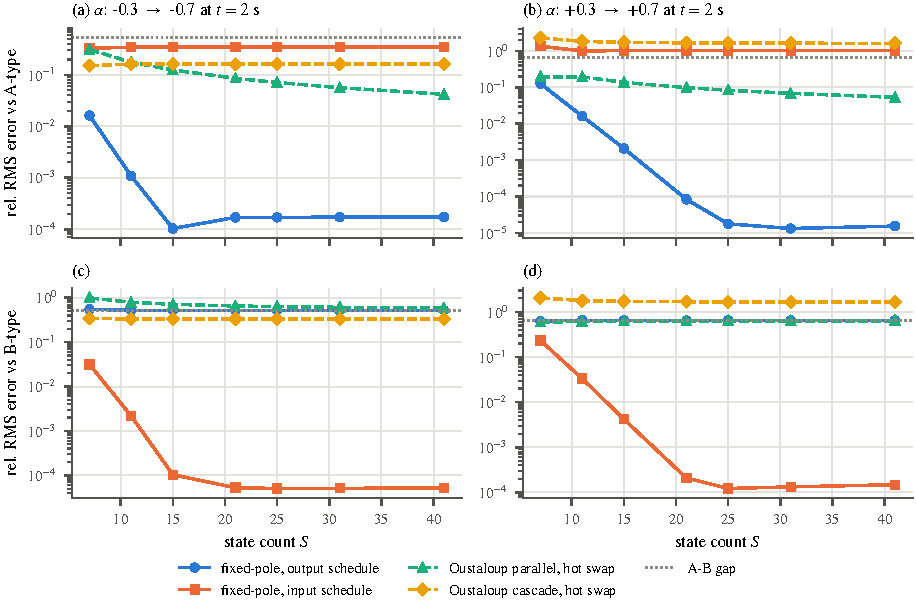
\includegraphics[width=\textwidth]{figs/fig_definition.pdf}
\caption{Continuous time, unit step, one order switch at $t=2$\,s. Relative RMS error after the switch against the A-type (top) and B-type (bottom) closed forms versus state count. The dotted line is the distance between the two definitions. Every series has its own marker and line style}\label{fig:definition}
\end{figure}

\begin{table}[t]
\caption{Continuous time, step input: relative RMS error after a single switch. FP-out and FP-in are the fixed-pole bank with output and input schedule; Ou-par and Ou-cas are the hot-swapped Oustaloup forms. Arrows show $S=15\to41$; the cascade column is at $S=41$}\label{tab:e1}
\footnotesize\setlength{\tabcolsep}{4pt}
\begin{tabular}{@{}lccccc@{}}
\toprule
$\alpha_1\to\alpha_2$ & A--B gap & FP-out vs A & FP-in vs B & Ou-par vs A & Ou-cas, A / B\\
\midrule
$-0.3\to-0.7$ & 0.52 & $1.0\mathrm{e}{-4}\to1.7\mathrm{e}{-4}$ & $1.0\mathrm{e}{-4}\to5.1\mathrm{e}{-5}$ & $0.12\to0.042$ & 0.16 / 0.33\\
$+0.3\to+0.7$ & 0.65 & $2.1\mathrm{e}{-3}\to1.5\mathrm{e}{-5}$ & $4.2\mathrm{e}{-3}\to1.5\mathrm{e}{-4}$ & $0.14\to0.053$ & 1.6 / 1.7\\
$-0.5\to+0.5$ & 0.81 & $1.1\mathrm{e}{-3}\to4.3\mathrm{e}{-5}$ & $5.1\mathrm{e}{-4}\to3.1\mathrm{e}{-5}$ & $0.23\to0.085$ & 4.6 / 1.6\\
$+0.5\to-0.5$ & 1.35 & $9.8\mathrm{e}{-5}\to3.4\mathrm{e}{-5}$ & $9.4\mathrm{e}{-4}\to8.0\mathrm{e}{-6}$ & $0.25\to0.080$ & 0.24 / 0.87\\
\botrule
\end{tabular}
\footnotetext{On the fixed band $[10^{-3},10^{5}]$\,rad/s used here, the fixed-pole bank reaches its tail floor near $S=15$. The rule of Sect.~\ref{sec:design} chooses the band from the tolerance instead.}
\end{table}

\paragraph{Discrete time.} The discrete bank (32 modes and the delay mode) was compared with the GL definitions over 7 order profiles and 3 inputs (step, white noise, multisine). The total error of the output schedule against the A-type was $2.5\times10^{-6}$ to $2.0\times10^{-3}$, and that of the input schedule against the B-type $1.9\times10^{-6}$ to $1.6\times10^{-3}$. Smooth derivative orders are included, so the continuous-time failure disappears. Table~\ref{tab:e1b} gives the definitional errors. For the bank they are zero, or zero to rounding, as Proposition~\ref{prop:structure} predicts. For the hot-swapped Oustaloup forms they are not, and the cascade form reaches $3\times10^{3}$.

\begin{table}[t]
\caption{Discrete time, piecewise-constant orders: definitional error (distance from the realization's own type). DFP is the discrete fixed-pole bank; the Oustaloup forms have $N=15$ ($S=31$)}\label{tab:e1b}
\begin{tabular}{@{}lcc@{}}
\toprule
Realization & vs own A-type & vs own B-type\\
\midrule
DFP, output schedule & 0 (exact) & equals the A--B gap\\
DFP, input schedule & equals the A--B gap & $\le10^{-14}$\\
Oustaloup parallel, hot swap & $4\times10^{-6}$ to $0.13$ & $7\times10^{-3}$ to $1.0$\\
Oustaloup cascade, hot swap & $7\times10^{-3}$ to $3.0\times10^{3}$ & $0.03$ to $4.8\times10^{2}$\\
\botrule
\end{tabular}
\end{table}

\subsection{Can a state map repair a moving-pole realization?}\label{sec:res-maps}

\paragraph{Setup.} For six single switches (at sample 2000, window 2000), we fitted $\Phi$ by truncated least squares on a mixed training ensemble of 4 classes with 200 inputs each (white, piecewise-constant, multisine, Brownian). We tested on fresh ensembles of 150 inputs per class and on a unit step, sweeping the truncation threshold. Besides the most accurate map, we report a robust \emph{minimum-norm} map: the map of smallest norm whose validation error is within twice the best. The maps were then rounded to float32 and to 24-bit fixed point.

\paragraph{Results.} Figure~\ref{fig:maps} and Table~\ref{tab:e2} report the worst case over the switches and the input classes. In float64 the error falls from $0.14$ (parallel, hot swap) and $1.1\times10^4$ (cascade, hot swap) to $1.7\times10^{-7}$ and $6.2\times10^{-7}$ at $S=31$. The map is, however, a dense $S\times S$ matrix, with norm between $10^3$ and $5\times10^4$ even for the minimum-norm choice. Rounded to 24 bits, the map loses 3.5 to 4.3 orders of magnitude of accuracy in the parallel form and 7.4 to 9.1 in the cascade form for $S\ge21$. In the cascade form the 24-bit error exceeds 1, and even float32 rounding raises it to $0.26$--$0.81$ for $S\ge15$.

With a smooth derivative order quantized to 41 levels (80 grid crossings, parallel form), a chain of maps reduced the step-input error from $4.1\times10^{-2}$ to $1.2\times10^{-4}$ ($S=15$). The fixed-pole bank needs no map, and its definitional error is exactly zero. For the $P=1024$ order levels of Sect.~\ref{sec:hw}, maps between neighbouring levels alone would need about 56\,Mbit of storage at $S=33$ and 25 bits per entry, against 0.78--1.08\,Mbit for the whole coefficient table of the bank.

\begin{figure}[t]
\centering
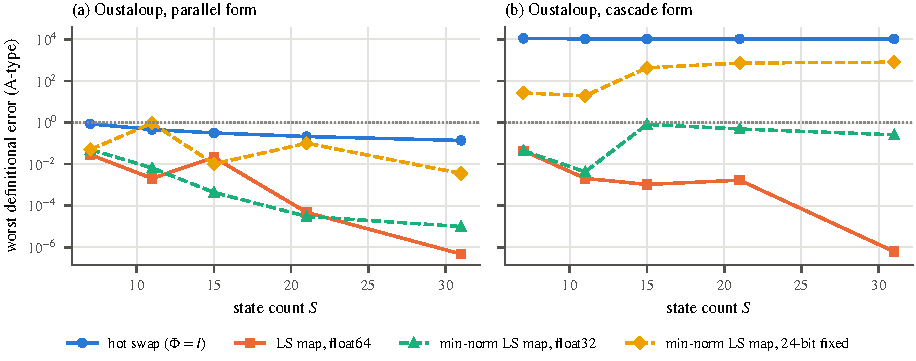
\includegraphics[width=\textwidth]{figs/fig_maps.pdf}
\caption{Worst definitional error (A-type) after one switch, over six switches and five input classes including the step. Hot swap versus least-squares state maps in float64, and the minimum-norm map rounded to float32 and to 24-bit fixed point. The dotted line marks an error of 1}\label{fig:maps}
\end{figure}

\begin{table}[t]
\caption{State maps for the Oustaloup forms: worst A-type definitional error over 6 switches and 5 input classes (including the step), and the largest norm of the minimum-norm map}\label{tab:e2}
\footnotesize\setlength{\tabcolsep}{4pt}
\begin{tabular}{@{}llccccc@{}}
\toprule
 & & & & \multicolumn{3}{c}{minimum-norm map}\\
\cmidrule(l){5-7}
$S$ & form & hot swap & LS, float64 & float64 ($\|\Phi\|_2$) & float32 & 24-bit\\
\midrule
7  & parallel & 0.86 & $2.8\mathrm{e}{-2}$ & $5.0\mathrm{e}{-2}$ ($3\mathrm{e}{4}$) & $5.0\mathrm{e}{-2}$ & $5.0\mathrm{e}{-2}$\\
15 & parallel & 0.32 & $2.1\mathrm{e}{-2}$ & $4.4\mathrm{e}{-4}$ ($5\mathrm{e}{4}$) & $4.3\mathrm{e}{-4}$ & $1.0\mathrm{e}{-2}$\\
31 & parallel & 0.14 & $4.7\mathrm{e}{-7}$ & $1.7\mathrm{e}{-7}$ ($5\mathrm{e}{3}$) & $9.8\mathrm{e}{-6}$ & $3.6\mathrm{e}{-3}$\\
7  & cascade & $1.1\mathrm{e}{4}$ & $4.4\mathrm{e}{-2}$ & $4.4\mathrm{e}{-2}$ ($9\mathrm{e}{2}$) & $4.4\mathrm{e}{-2}$ & $2.7\mathrm{e}{1}$\\
15 & cascade & $1.1\mathrm{e}{4}$ & $1.0\mathrm{e}{-3}$ & $3.2\mathrm{e}{-4}$ ($8\mathrm{e}{3}$) & $8.1\mathrm{e}{-1}$ & $4.3\mathrm{e}{2}$\\
31 & cascade & $1.1\mathrm{e}{4}$ & $6.2\mathrm{e}{-7}$ & $6.2\mathrm{e}{-7}$ ($4\mathrm{e}{4}$) & $2.6\mathrm{e}{-1}$ & $8.1\mathrm{e}{2}$\\
\botrule
\end{tabular}
\footnotetext{The fixed-point test rounds $\Phi$ to a single Q format; per-row scaling might do better. The fixed-pole bank needs $\Phi=I$ and has zero definitional error.}
\end{table}

\subsection{Design rule on a sealed holdout}\label{sec:res-rule}

\paragraph{Term validation.} Each term of Sect.~\ref{sec:design} was first isolated by making the other two negligible (Fig.~\ref{fig:rule}a,b). The ratio of measured to predicted error was 0.49--1.05 in discrete time ($n=45$) and 0.99--1.01 in continuous time ($n=66$). The model never underestimates a term by more than 5\,\%.

\paragraph{Holdout.} We drew 400 random specifications (200 discrete, 200 continuous) from a fixed seed:
\begin{itemize}
\item $\eps\in[10^{-5},10^{-2}]$;
\item $R\in[10^2,10^5]$, or bands of 0.5 to 6 decades;
\item random order ranges inside $[-0.95,0.95]$.
\end{itemize}
The specifications were written with their SHA-256 digest before any evaluation and then evaluated once. Every specification was met: 200 of 200 in both domains. The one-sided 95\,\% Clopper--Pearson lower bound~\cite{clopper1934} on the pass rate is 98.5\,\% for each domain. The achieved error was a median 0.41 (discrete) and 0.50 (continuous) of the requested $\eps$, with maxima 0.67 and 0.72. Let $K_{\min}$ be the smallest $K$ on the same grid endpoints that still meets $\eps$, found by bisection. The rule exceeded it by a median of one mode and at most three. Table~\ref{tab:K} lists typical sizes: each decade of memory adds about three modes, and each decade of accuracy seven to ten.

\begin{figure}[t]
\centering
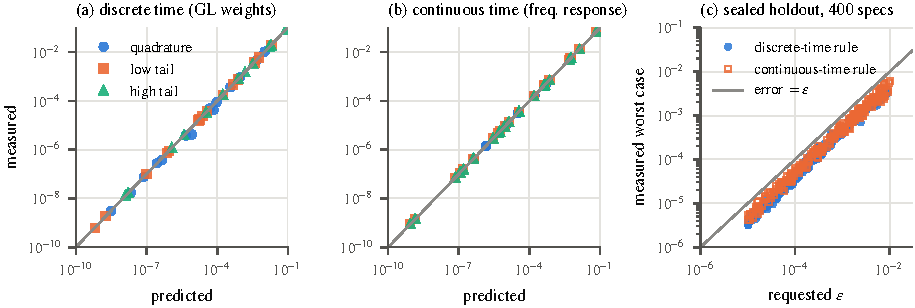
\includegraphics[width=\textwidth]{figs/fig_rule.pdf}
\caption{Analytic error model. (a, b) Each term isolated, measured against predicted. (c) Sealed holdout: measured worst-case error against the requested tolerance for 400 random specifications}\label{fig:rule}
\end{figure}

\begin{table}[t]
\caption{Bank size $K$ from the rule for $\alpha\in[-0.9,0.9]$. Discrete time: memory length $R$ in samples (plus the delay mode). Continuous time: band width in decades}\label{tab:K}
\begin{tabular}{@{}lcccccc@{}}
\toprule
 & \multicolumn{3}{c}{discrete time, $R$} & \multicolumn{3}{c}{continuous time, band}\\
\cmidrule(lr){2-4}\cmidrule(lr){5-7}
$\eps$ & $10^3$ & $10^4$ & $10^5$ & 2 dec. & 4 dec. & 6 dec.\\
\midrule
$10^{-2}$ & 14 & 17 & 19 & 11 & 14 & 16\\
$10^{-3}$ & 21 & 24 & 27 & 18 & 22 & 26\\
$10^{-4}$ & 29 & 32 & 36 & 27 & 32 & 37\\
$10^{-5}$ & 38 & 42 & 46 & 38 & 44 & 50\\
\botrule
\end{tabular}
\end{table}

\subsection{Four types from one bank}\label{sec:res-types}

\paragraph{Definitions.} The literal recursions~\eqref{eq:D},~\eqref{eq:E} agree with $\WA(-\alpha)^{-1}$ and $\WB(-\alpha)^{-1}$ to $1.4\times10^{-13}$. The dual compositions ($\mathrm A\circ\mathrm D$, $\mathrm D\circ\mathrm A$, $\mathrm B\circ\mathrm E$, $\mathrm E\circ\mathrm B$) return the identity to $10^{-12}$. The non-dual compositions (A$\circ$A, B$\circ$B, A$\circ$B, B$\circ$A, A$\circ$E, B$\circ$D, D$\circ$E, D$\circ$D) differ from the identity by $10^{-2}$ to $2.4\times10^{3}$.

\paragraph{Bank.} A bank designed for $\eps=10^{-5}$, $|\alpha|\le0.95$ and $R=4000$ ($K=41$) was run in all four types over 5 order profiles and 3 inputs (Table~\ref{tab:e4}). The error against the literal definitions is at most $6.9\times10^{-5}$. The definitional error is at rounding level, and the duality holds in the bank to $2\times10^{-14}$. The largest output errors occur for derivatives with smooth inputs, where the weights cancel (Corollary~\ref{cor:bound}).

\begin{table}[t]
\caption{One bank ($K=41$) in four types: error against the literal GL definitions (15 cases), and against the bank's own type (the 12 piecewise-constant cases)}\label{tab:e4}
\begin{tabular}{@{}lcc@{}}
\toprule
Type & vs literal definition & vs own type (definitional)\\
\midrule
A & $9.5\times10^{-8}$ to $6.9\times10^{-5}$ & $\le2.6\times10^{-14}$\\
B & $3.1\times10^{-8}$ to $1.2\times10^{-5}$ & $\le1.0\times10^{-14}$\\
D & $2.0\times10^{-8}$ to $6.5\times10^{-5}$ & $\le2.3\times10^{-14}$\\
E & $2.2\times10^{-8}$ to $5.5\times10^{-5}$ & $\le2.8\times10^{-13}$\\
\botrule
\end{tabular}
\end{table}

\paragraph{Inverse stability.} Over the 200 discrete-time holdout designs, checked at 25 orders spanning each design range, the inverse was stable at every order in 200/200 designs with the DC floor and in 101/200 without it. Figure~\ref{fig:types}b shows a D-type integral of order $0.95$ driven by white noise for $2\times10^5$ samples ($\eps=10^{-2}$, $R=1000$, $K=15$). Without the floor the output RMS grows to $1.9\times10^{21}$; with the floor it stays below $0.36$.

\paragraph{Which type does a hot swap implement?} Using the own-type references, we asked which of the four types each hot-swapped realization is closest to, over 8 cases (four piecewise-constant order profiles, step and white-noise inputs) for $N=7$ and $N=15$:
\begin{itemize}
\item the fixed-pole bank is closest to A (output schedule) or B (input schedule) in all cases, at distances $\le2.1\times10^{-14}$;
\item the parallel Oustaloup form is closest to the A-type in all cases, at distances up to $0.42$;
\item for the cascade form with $\omega_h=10^3$\,rad/s, the closest type is A, B, D and E in two cases each, so the cascade has no consistent type; with $\omega_h=10^5$\,rad/s it is A or B, at distances up to $1.3\times10^{3}$;
\item with $\omega_h=10^5$\,rad/s, above the Nyquist frequency, the zero-order-hold members of the integral approximations have zeros outside the unit circle (moduli 3 to 41), and their own D- and E-types cannot even be formed in 6 of 8 cases.
\end{itemize}

\paragraph{Relaxation equations.} For $\Op{T}{\alpha}y+\lambda y=u$ (Remark~\ref{rem:relax}; $K=40$, $n=4000$), the bank matched the triangular GL solutions to $1.7\times10^{-5}$ ($\lambda=1$) and $4.9\times10^{-7}$ ($\lambda=100$). The solutions of different types differed by up to $0.40$ for $\lambda=1$ (Fig.~\ref{fig:types}a), so the choice of type changes the solution visibly. For $\lambda=100$ the term $\lambda y$ dominates and the types differ by at most $0.02$.

\begin{figure}[t]
\centering
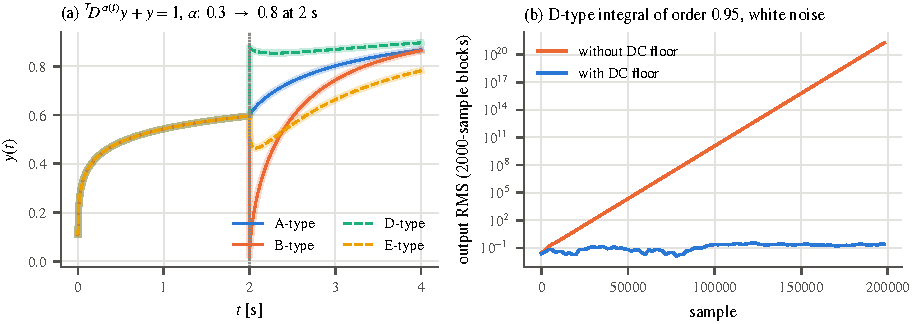
\includegraphics[width=\textwidth]{figs/fig_types.pdf}
\caption{(a) Relaxation equation of all four types with one bank; thin lines are the bank, wide light lines the triangular GL solutions. (b) D-type integral of order 0.95 (inverse of the 0.95 derivative bank) on white noise, with and without the DC floor}\label{fig:types}
\end{figure}

%% =====================================================================
\section{Fixed-point realization}\label{sec:hw}

The design point is $R=4000$, $\eps=10^{-4}$ and $|\alpha|\le0.95$, giving $K=32$ plus the delay mode. Orders come from a grid of $P=1024$ levels, $\alpha_i=0.95\,(2i/(P-1)-1)$, so $\Delta\alpha=1.9\times10^{-3}$.

\subsection{Arithmetic in sample units}

The core runs in sample units ($\Ts=1$), where $\gh_0=1$ for every order. The inversion~\eqref{eq:inverse} then needs no divider: $v_n=x_n-\eta_n$. Physical units follow from one gain $\Ts^{-\alpha_n}$, applied at the output for the A- and E-types and at the input for the B- and D-types. This follows directly from~\eqref{eq:A}--\eqref{eq:E}; for the E-type, substitute $z_n=\Ts^{-\alpha_n}\zeta_n$.

The number formats are as follows:
\begin{itemize}
\item \emph{Signals:} $W_S$-bit two's complement with $F$ fractional bits.
\item \emph{States:} $W_{ST}=W_S+13$ bits. Each mode stores its state scaled by a power of two $2^{G_k}$ (one gain per schedule) so that its own bound uses the full word. Without this scaling, the input-scheduled slow modes lose their increments $c_kv_n$, which lie far below the signal LSB; the B- and E-type errors were then $2\times10^{-2}$ to $0.66$.
\item \emph{Coefficients:} a $W_M$-bit mantissa with a 7-bit shift.
\end{itemize}
Products are rounded as $\mathrm{mulsh}(a,M,S)=(aM+2^{S-1})\gg S$. Algorithm~\ref{alg:core} gives one sample of the core in exact arithmetic; the bit-accurate golden model and the RTL use the same sequence with the formats above.

\begin{algorithm}[t]
\caption{One sample of the bank, all four types. In hardware the coefficient row is a ROM word addressed by the order index (mirrored for D and E), so an order or type change costs nothing}\label{alg:core}
\begin{algorithmic}[1]
\Require type $T\in\{\mathrm{A,B,D,E}\}$, order $\alpha_n$, input $x_n$; states $s_0,\dots,s_{K-1},\sd$
\State $a\gets\alpha_n$ if $T\in\{\mathrm{A,B}\}$, else $a\gets-\alpha_n$; read $(\cd,c_0,\dots,c_{K-1})$ for order $a$
\If{$T\in\{\mathrm{A,D}\}$} \Comment{output schedule}
  \State $\eta\gets\cd\,\sd+\sum_k c_k s_k$
\Else \Comment{input schedule}
  \State $\eta\gets\sd+\sum_k s_k$
\EndIf
\If{$T\in\{\mathrm{A,B}\}$} $v\gets x_n$;\ \ $y_n\gets v+\eta$
\Else\ $v\gets x_n-\eta$;\ \ $y_n\gets v$ \Comment{no divider in sample units}
\EndIf
\If{$T\in\{\mathrm{A,D}\}$} $s_k\gets\theta_k s_k+v$;\ \ $\sd\gets v$
\Else\ $s_k\gets\theta_k s_k+c_k v$;\ \ $\sd\gets\cd v$
\EndIf
\end{algorithmic}
\end{algorithm}

\subsection{Dynamic range: two operating envelopes}

For $|x|\le1$ over $4000$ samples, the frozen-order $\ell_1$ bound on the output is $2696$. For the A-type this bound holds under any switching, because each output uses the weights of a single order; for the B-type the switching stress tests stayed within it. For the D- and E-types, switching from an integral to a derivative order drives the output to $2.2\times10^6$ under a DC input, 820 times the frozen-order bound. The new inverse acts on a history that has grown under the old order. This is the behaviour of the recursive definitions themselves, not an artefact of the bank. We therefore size two envelopes with a factor-two margin: 14 integer bits for the forward types only (A/B), and 24 integer bits for all four types (A/B/D/E).

\subsection{Quantization and inverse stability}\label{sec:hw-stab}

Quantization can undo the DC floor. Coefficients and pole steps are dyadic rationals, so the signs of $\Hh_q(\pm1)$ of every quantized ROM row can be evaluated exactly in rational arithmetic, which we did. With the floating-point floor alone:
\begin{itemize}
\item in the A/B configuration, 64 of the 512 positive-order rows have $\Hh_q(1)\le0$, the worst having its dominant inverse pole at $1+4.8\times10^{-6}$ (e-folding time $2.1\times10^5$ samples);
\item in the A/B/D/E configuration, 51 of 512 rows have $\Hh_q(1)\le0$, the worst ($\alpha=0.855$) having its pole at $1+1.9\times10^{-9}$ (e-folding time $5.2\times10^{8}$ samples, about 9 minutes at 1\,MS/s).
\end{itemize}
$\Hh_q(-1)$ was positive in every row. The \emph{quantization-aware} DC floor raises the delay mantissa in LSB steps until $\Hh_q(1)$ is at least the floating-point value $\Hh(1)$. It brings both counts to zero without any measurable change in accuracy.

\subsection{Word length}

We swept $W_S\in\{32,\dots,56\}$ and $W_M\in\{16,18,25,32\}$ (Fig.~\ref{fig:wordlength}). The test set comprised 3 order profiles (random piecewise, a new order every sample, a sign-changing switch), 3 inputs, and all types of the envelope. A configuration was accepted if, for every type, its error against the literal definition was at most the floating-point bank's error plus $0.1\eps$. The smallest accepted configurations were:
\begin{itemize}
\item A/B: $W_S/W_{ST}/W_M=36/49/16$;
\item A/B/D/E: $48/61/25$.
\end{itemize}
With an 18-bit mantissa the D- and E-types stall near $10^{-3}$, because the inversion is ill-conditioned: the low-frequency gain of a derivative bank is about $R^{-\alpha}$. The floating-point bank itself has D- and E-type output errors up to $6\times10^{-4}$ at this design point, although its weight error is $10^{-4}$. This is the cancellation effect of Corollary~\ref{cor:bound}, amplified by the inversion.

\begin{figure}[t]
\centering
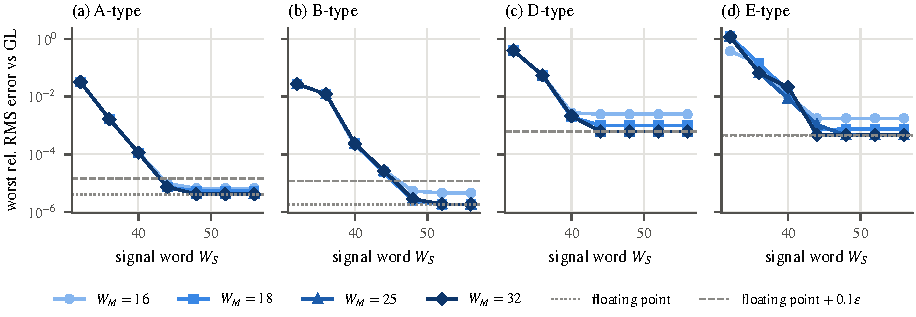
\includegraphics[width=\textwidth]{figs/fig_wordlength.pdf}
\caption{Word length, A/B/D/E envelope: worst relative RMS error against the literal definitions versus signal word $W_S$ (state word $W_S+13$), for four mantissa widths. Dotted: floating-point bank; dashed: acceptance limit}\label{fig:wordlength}
\end{figure}

\subsection{RTL, parity and resources}

The core (\texttt{vo\_bank\_core.v}) is a non-pipelined, time-multiplexed state machine with synchronous coefficient, pole and gain ROMs. It takes $4K+8=136$ clock cycles per sample. Order index and type are inputs with every sample. An order change only changes a ROM address: there is no reload and no extra cycle.

The test vectors cover constant, piecewise and per-sample orders, sign-changing switches, full-scale inputs, and type changes at run time. The type changes exercise the datapath; a type change is not itself a VO operation. Icarus Verilog simulation matched the golden model bit for bit on all 94\,208 vectors (31\,744 for A/B, 62\,464 for A/B/D/E). Verilator lint reported only intentional width extensions and truncations. Table~\ref{tab:rtl} lists Yosys estimates for a 7-series FPGA.

\begin{table}[t]
\caption{RTL configurations: bit-exact parity with the golden model and Yosys \texttt{synth\_xilinx} (xc7) resource estimates. Vivado results and $f_{\max}$ are pending}\label{tab:rtl}
\begin{tabular}{@{}lcccccc@{}}
\toprule
Envelope & $W_S/W_{ST}/W_M$ & vectors (mismatches) & LUT & FF & DSP48E1 & RAMB36 eq.\\
\midrule
A/B & 36/49/16 & 31\,744 (0) & 4\,171 & 1\,882 & 11 & 22\\
A/B/D/E & 48/61/25 & 62\,464 (0) & 6\,009 & 2\,360 & 29 & 29.5\\
\botrule
\end{tabular}
\end{table}

\pending{Board measurements (to be added): bitstream-level parity on the same vectors, Vivado utilization and $f_{\max}$, sample rate $f_{\max}/136$, per-sample order changes, and a long run ($\ge10^7$ samples) of the D-type at the worst quantized row. These will be measured with the new core; no measurement from~\cite{tcas_submission} is reused.}

%% =====================================================================
\section{Application: streaming multifractional Brownian motion}\label{sec:mbm}

Multifractional Brownian motion lets the Hurst exponent vary in time~\cite{peltier1995}, and its definitions are in general not equivalent~\cite{stoev2006}. The Riemann--Liouville form (RL-mBm)~\cite{lim2001,muniandy2001} is a VO integral of white noise of order $H(t)+\tfrac12$, with the current order applied to the whole past. It is thus an A-type integral. Applying the order at the time each increment enters gives the B-type variant. Up to the discretization of the kernel and a per-increment factor $\sqrt{2H_j}\,\Gamma(H_j+\tfrac12)$, this is the memory-multifractional Brownian motion (MMFBM) of Wang et al.~\cite{wang2023mmfbm}, $X(t)=\int_0^t\sqrt{\alpha(s)}\,(t-s)^{(\alpha(s)-1)/2}\,\mathrm dB(s)$ with $\alpha=2H$. The input-scheduled bank applies that factor as a gain on each input sample. Related constructions in which a change of $H$ acts only on new increments are the nonhomogeneous fractional integration of Surgailis~\cite{surgailis2008}, the integrated fractional white noise of Sly~\cite{sly2007}, the variable-Hurst fBm of Ryvkina~\cite{ryvkina2015} and the incremental mBm of \'Sl\c{e}zak and Metzler~\cite{slezak2023}. VO operators have been used to synthesize multifractional Gaussian noise before~\cite{sheng2011}, and simulation methods for mBm include~\cite{chan1998}. Exact methods for stationary Gaussian processes such as circulant embedding~\cite{wood1994} rely on stationarity and do not apply directly when $H$ varies.

In sample units, the discrete processes are
\[
X^{\mathrm A}_n=\sum_r g_r(-a_n)\,\xi_{n-r},\qquad X^{\mathrm B}_n=\sum_j g_{n-j}(-a_j)\,\xi_j,\qquad a_n=H_n+\tfrac12,
\]
with i.i.d.\ standard normal $\xi$. For $H>\tfrac12$ the order exceeds 1, outside the range of the bank. An integer integration can be split off exactly, but only in the right place:

\begin{proposition}[Integer split]\label{prop:split}
Let $\Sigma$ denote the cumulative sum. Then
\[
\Op{A}{-a}\xi=\Op{A}{-(a-1)}(\Sigma\xi),\qquad \Op{B}{-a}\xi=\Sigma\big(\Op{B}{-(a-1)}\xi\big).
\]
\end{proposition}
\begin{proof}
$(1-z^{-1})^{-a}=(1-z^{-1})^{-(a-1)}(1-z^{-1})^{-1}$ gives $w_m(-a)=\sum_{i=0}^{m}w_i(-(a-1))$ for every fixed $a$. For the A-type, apply this at the fixed order $a_n$ of output sample $n$ and exchange the sums. For the B-type, sample $j$ keeps its order $a_j$:
\[
\sum_{j\le n}\sum_{i\le n-j}w_i\big(-(a_j-1)\big)\xi_j=\sum_{m\le n}\sum_{j\le m}w_{m-j}\big(-(a_j-1)\big)\xi_j .
\]
The right-hand side is the cumulative sum of $\Op{B}{-(a-1)}\xi$.
\end{proof}

The reversed orders are not exact: the relative errors are 0.1 to 1.3 in our tests. With the split, one bank of order $\tfrac12-H$, which satisfies $|\tfrac12-H|<\tfrac12$, covers all of $0<H<1$. It crosses $H=\tfrac12$ seamlessly because the order $0$ is exact in the bank.

\paragraph{Results.} Table~\ref{tab:mbm} and Fig.~\ref{fig:mbm} summarize the results. The bank was designed by the rule for $\eps=10^{-4}$ and $0.05\le H\le0.95$, giving $K=22$, 24 and 26 for $n=1024$, 4096 and 16\,384.

Second-order statistics were computed exactly, without Monte Carlo, from the $n\times n$ weight matrix of the generator. The variance agreed with the exact formula to $3.1\times10^{-5}$ and the covariance to $1.7\times10^{-6}$.

The local Hurst exponent was estimated by generalized quadratic variations~\cite{istas1997,coeurjolly2005}; see~\cite{bardet2013} for multifractional Gaussian processes. For constant $H$ the estimator itself has a bias of $+0.06$ at $H=0.2$ and a standard deviation of $0.06$ (window 1024). For varying $H$ its mean followed $H(t)$ with RMSE $0.014$ to $0.036$, equally for both types.

The two types differ sharply at a jump of $H$ from $0.3$ to $0.8$. The A-type variance jumps from 119 to $1.5\times10^5$, and the path is discontinuous: the squared increment at the jump is $1.3\times10^5$ times the typical one. The B-type is continuous (ratio 1.0), in line with the behaviour reported for MMFBM and incremental mBm~\cite{wang2023mmfbm,slezak2023}. Which definition to use is therefore a modelling decision with visible consequences, as also argued in~\cite{wang2023mmfbm}. The bank makes either choice available at the same cost.

\begin{table}[t]
\caption{Streaming mBm with the fixed-pole bank}\label{tab:mbm}
\small
\begin{tabular}{@{}>{\raggedright\arraybackslash}p{0.44\textwidth}>{\raggedright\arraybackslash}p{0.52\textwidth}@{}}
\toprule
Quantity & Result\\
\midrule
integer split, correct order (A first, B last) & $\le9\times10^{-15}$\\
integer split, reversed order & $0.1$ to $1.3$\\
path vs literal GL, same noise & A $\le1.9\times10^{-6}$, B $\le2.4\times10^{-6}$\\
exact variance / covariance ($n=2048$) & $\le3.1\times10^{-5}$ / $\le1.7\times10^{-6}$ (Frobenius)\\
local Hurst tracking, varying $H$ (400 paths) & RMSE of mean 0.014 to 0.036, A and B alike\\
variance before/after a jump of $H$ from $0.3$ to $0.8$ & A $119\to1.5\times10^{5}$; B $119\to119$\\
cost per sample & bank 47 to 55 MACs ($n$-independent); direct GL $n/2$ on average\\
fixed-point core A/B (36/49/16), vs float & A $1.8\times10^{-5}$, B $8.9\times10^{-4}$\\
fixed-point core A/B/D/E (48/61/25), vs float & A $3.8\times10^{-6}$, B $1.2\times10^{-4}$\\
\botrule
\end{tabular}
\end{table}

\paragraph{Hardware.} The cores of Sect.~\ref{sec:hw} generate the same processes bit-exactly from integer noise. For the A-type, the accumulator sits in front of the core and is exact (an integer sum), so the small A/B core suffices. For the B-type, the accumulator follows the core and integrates its low-frequency rounding errors. The B-type therefore benefits from the wider configuration (Table~\ref{tab:mbm}, last two rows). Input scales were $2^{-9}$ for A and $0.25$ for B, chosen to keep the accumulated A-type input within the signal range.

\begin{figure}[t]
\centering
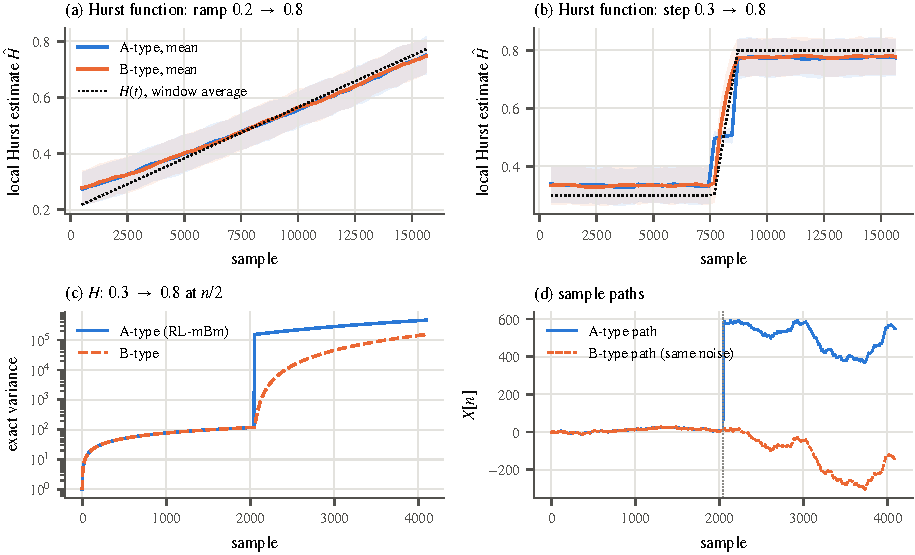
\includegraphics[width=\textwidth]{figs/fig_mbm.pdf}
\caption{Streaming mBm. (a, b) Local Hurst estimates (mean $\pm$ one standard deviation over 400 paths) for a ramp and a step of $H$. (c) Exact variance of the A-type (RL-mBm) and B-type processes for a jump of $H$ at $n/2$. (d) Sample paths driven by the same noise}\label{fig:mbm}
\end{figure}

%% =====================================================================
\section{Discussion and limitations}\label{sec:discussion}

\paragraph{Scope of the guarantees.} Proposition~\ref{prop:structure} and Corollary~\ref{cor:bound} hold for every order sequence. Proposition~\ref{prop:stability} is a statement about each \emph{frozen} order. The recursive types under switching form a switched linear system $F-b\,c(\alpha_n)^{\top}/\gh_0$, whose stability under arbitrary switching is not implied by the stability of each member. In all our tests the switched D- and E-types stayed bounded, within the stress envelope of Sect.~\ref{sec:hw}, but we have no proof for arbitrary switching.

\paragraph{Output versus weight error.} The rule guarantees the relative weight error. For derivatives, and even more for the inverses, the output error can exceed it: by up to a factor of seven for the bank of Sect.~\ref{sec:res-types}, and up to six for the D- and E-types at the design point of Sect.~\ref{sec:hw}. An output-level rule would have to account for the input class.

\paragraph{Order range.} The bank covers $-1<\alpha<1$. Larger orders follow from integer splits such as Proposition~\ref{prop:split}, which must be placed according to the type.

\paragraph{Fixed point.} We used a single Q format per signal. Block floating point could reduce the D/E word lengths, which are dominated by the switching envelope.

\paragraph{Hardware.} The core is not pipelined. A pipelined version could approach $K$ plus a few cycles per sample. Resources are synthesis estimates, and the board measurements are pending.

\paragraph{Literature search.} The review of Sect.~\ref{sec:related} used Crossref and arXiv. \pending{TODO: repeat the documented queries in Scopus and Web of Science before submission.}

%% =====================================================================
\section{Conclusion}\label{sec:conclusion}

For a finite-dimensional realization of a variable-order operator, the definition it implements is a property of its structure. If the poles move with the order, no state map can make a switched realization exact for the A- or B-type. If the poles are fixed and the order sits in the output or input weights, the realization is the A- or B-type for every order sequence, up to the frozen-order quadrature error. Inverting the same bank gives the D- and E-types with exact duality. The Beta-integral representation makes this exact in discrete time. An analytic rule sizes the bank, and a DC floor, tested by an exact sign, keeps every inverse stable, also after quantization. In hardware the order and the type become a ROM address that can change at every sample. Streaming multifractional Brownian motion shows that the choice between the A- and B-type is a modelling decision with visible consequences, which the bank makes explicit.

\backmatter

\bmhead{Acknowledgements}
\pending{TODO.}

\section*{Declarations}

\begin{itemize}
\item \textbf{Funding:} \pending{TODO.}
\item \textbf{Competing interests:} The authors declare no competing interests. \pending{TODO: confirm.}
\item \textbf{Data availability:} All results reported in this paper are produced by the scripts in the accompanying repository, with fixed seeds; the result files are included.
\item \textbf{Code availability:} \pending{TODO: public repository URL or archive DOI.} The repository contains the Python library, the experiments, the Verilog core, the testbench and the board test bundle.
\item \textbf{Author contributions:} \pending{TODO.}
\item \textbf{Relation to other work:} A constant-order FPGA approximation by the same authors is under review elsewhere~\cite{tcas_submission}. The present paper uses different structures (order-independent poles), a different design rule (analytic, fit-free) and a new core. It reuses no figure, table, text or measurement from that work.
\end{itemize}

\begin{appendices}

\section{Proof of Theorem~\ref{thm:necessity}}\label{app:necessity}

Write $\mathcal C_i=[b_i,F_ib_i,\dots,F_i^{S-1}b_i]$ and $\mathcal O_i=[c_i,F_i^{\top}c_i,\dots,(F_i^{\top})^{S-1}c_i]^{\top}$, both invertible by minimality~\cite{kailath1980}.

(a) For $n\ge m$ the switched output is $d_2v_n+c_2^{\top}F_2^{\,n-m}\Phi x_1[m]+c_2^{\top}\sum_{m\le j<n}F_2^{\,n-1-j}b_2v_j$. The response of $\Sigma_2$ to the whole input differs from it only by $\Phi x_1[m]$ being replaced by $x_2[m]=\sum_{j<m}F_2^{\,m-1-j}b_2v_j$. Equality for all inputs and all $n\ge m$ means $c_2^{\top}F_2^{\,k}(\Phi x_1[m]-x_2[m])=0$ for all $k\ge0$. By observability this holds if and only if $\Phi x_1[m]=x_2[m]$ for every input history, that is, if and only if $\Phi F_1^{\,k}b_1=F_2^{\,k}b_2$ for $k=0,\dots,m-1$. Since $m\ge S+1$, this gives $\Phi\mathcal C_1=\mathcal C_2$, so $\Phi$ is invertible. It also gives $(\Phi F_1-F_2\Phi)F_1^{\,k}b_1=\Phi F_1^{\,k+1}b_1-F_2^{\,k+1}b_2=0$ for $k=0,\dots,S-1$, hence $(\Phi F_1-F_2\Phi)\mathcal C_1=0$ and $F_2=\Phi F_1\Phi^{-1}$. Conversely, if $F_2=\Phi F_1\Phi^{-1}$ and $b_2=\Phi b_1$, then $\Phi F_1^{\,k}b_1=F_2^{\,k}b_2$ for all $k$.

(b) The B-type behaviour requires that the stored state continue as in $\Sigma_1$: $c_2^{\top}F_2^{\,k}\Phi x=c_1^{\top}F_1^{\,k}x$ for all $k\ge0$ and every reachable $x$. By controllability every $x$ is reachable within $S\le m-1$ samples, so $\mathcal O_2\Phi=\mathcal O_1$. Then $\Phi$ is invertible, $c_2^{\top}=c_1^{\top}\Phi^{-1}$, and $\mathcal O_2(F_2\Phi-\Phi F_1)=0$ follows in the same way, so $F_2=\Phi F_1\Phi^{-1}$. The converse is immediate. \qed

\section{Proof of Proposition~\ref{prop:stability}}\label{app:stability}

$N$ has degree $K+1$. If $\cd=0$, then $z=0$ is a root of $N$; it cancels the delay pole and lies inside the disc. We give the argument for $\cd\neq0$; the case $\cd=0$ is the same with the pole at 0 removed.

(i) All residues are positive, so $\Hh$ decreases from $+\infty$ to $-\infty$ between consecutive poles of $\{0,\theta_0,\dots,\theta_{K-1}\}$. This gives $K$ roots in $(0,\max_k\theta_k)$. On $(\max_k\theta_k,\infty)$, $\Hh$ decreases from $+\infty$ to $g_0>0$, so there is no root there. On $(-\infty,0)$, $\Hh$ decreases from $g_0>0$ to $-\infty$, so there is exactly one root $z_*$. It lies in $(-1,0)$ if and only if $\Hh(-1)>0$.

(ii) Between consecutive $\theta_k$ the negative residues make $\Hh$ rise from $-\infty$ to $+\infty$, which gives $K-1$ roots. For $z>\max_k\theta_k$,
\[
z\Hh(z)=g_0z+\cd+\sum_k c_k\big(1+\theta_k/(z-\theta_k)\big)
\]
is strictly increasing from $-\infty$ to $+\infty$. Hence there is exactly one root there, and it is smaller than 1 if and only if $\Hh(1)>0$. If $\cd<0$, then $z\Hh(z)$ rises from $\cd<0$ at $z=0$ to $+\infty$ at $\min_k\theta_k^-$, giving the last root in $(0,\min_k\theta_k)$. If $\cd>0$, then $z\Hh(z)$ rises from $-\infty$ at $z\to-\infty$ to $\cd>0$ at $z=0$. Counting shows there is exactly one root $z_*<0$, with $z\Hh(z)<0$ for $z<z_*$. Hence $z_*>-1$ if and only if $-\Hh(-1)<0$, that is, $\Hh(-1)>0$. In all cases the $K+1$ roots are real, so no complex root can lie outside the disc.

(iii) Integral bank, order $-a$ with $0<a<1$. Since $\gh_1=\cd+\sum_kc_k$ and $\gh_2=\sum_kc_k\theta_k$,
\[
\Hh(-1)=g_0-\gh_1+\sum_k\frac{c_k\theta_k}{1+\theta_k}\ge g_0-\gh_1+\tfrac12\gh_2 .
\]
With $g_1=ag_0$, $g_2=\tfrac12a(1+a)g_0$ and relative errors at most $\delta=\tfrac13$, the right-hand side is at least $g_0(1-a)(6-a)/6>0$. Derivative bank, order $a$: here $\sum_k c_k\theta_k/(1+\theta_k)\ge\gh_2$ because $c_k<0$. Hence $\Hh(-1)\ge g_0-\gh_1+\gh_2$. With $g_1=-ag_0$ and $g_2=-\tfrac12a(1-a)g_0$, this is at least $g_0\big(1+\tfrac23a^2\big)>0$. \qed

\section{B-type step response}\label{app:stepB}

The B-type operator in continuous time processes each input sample with the kernel of its entry order: $y(t)=\int_0^t K(t-\tau,\alpha(\tau))u(\tau)\,\mathrm d\tau$ with $K(s,a)=\partial_sF(s,a)=s^{-a-1}/\Gamma(-a)$, taken in the finite-part sense for $a>0$. For $u=1$, let $G(\tau)=F(t-\tau,\alpha(\tau))$. Then
\[
\frac{\mathrm dG}{\mathrm d\tau}=-\partial_sF(t-\tau,\alpha(\tau))+\partial_aF(t-\tau,\alpha(\tau))\,\dot\alpha(\tau),
\]
so $y(t)=G(0)-G(t)+\int_0^t\partial_aF\,\dot\alpha\,\mathrm d\tau$. The finite part removes $G(t)=F(0^+,\alpha(t))$, and $G(0)=F(t,\alpha(0))$. This gives~\eqref{eq:stepB}. For a piecewise-constant order, $\dot\alpha$ is a sum of Dirac impulses and the integral becomes the stated finite sum. In the experiments the smooth case was evaluated by adaptive quadrature after the substitution $s=v^m$ with $m(1-\alpha_{\max})\ge2$, which removes the weak singularity at $s=0$.

\section{Large-lag alias term}\label{app:alias}

For large $r$ the integrand of~\eqref{eq:betax} is concentrated at $u=O(1/r)$, where $(1-e^{-u})^a\approx u^a$. Hence $f(x)\approx e^{(1+a)x}e^{-\rho e^x}$ with $\rho=r-a$. Its Fourier transform is $\hat f(\omega)=\Gamma(1+a-\mathrm i\omega)\rho^{-(1+a-\mathrm i\omega)}$, and $\hat f(0)=\Gamma(1+a)\rho^{-(1+a)}$ is the integral itself. The relative error of the infinite trapezoidal rule is $\sum_{k\neq0}\hat f(2\pi k/h)/\hat f(0)$, dominated by $k=\pm1$. Stirling's formula, $|\Gamma(1+a-\mathrm i\omega)|\sim\sqrt{2\pi}\,\omega^{a+1/2}e^{-\pi\omega/2}$, at $\omega=2\pi/h$ gives~\eqref{eq:Eq}. The result does not depend on $r$, which justifies the name large-lag term.

\end{appendices}

\bibliography{refs}

\end{document}
